\documentclass[a4paper,12pt]{fancy}
\usepackage{circuitikz}
\usepackage{graphicx}
\graphicspath{ {./images/} }
\usepackage[table]{xcolor}
\usepackage{pdflscape}
\usepackage{adjustbox}
\usepackage{pdfpages}
\usepackage[version=4]{mhchem}
\usepackage{tkz-euclide}
\definecolor{myyellow}{RGB}{254,241,24}
\definecolor{myorange}{RGB}{234,125,1}
\usepackage{tkz-euclide}
\usetkzobj{all}
\usetikzlibrary{calc,angles,quotes,decorations.markings}
\usetikzlibrary{shadings,shapes.geometric,calc, patterns, angles, quotes, arrows.meta, shapes, decorations.pathmorphing, decorations.shapes, decorations.text}
\tikzset{>=latex}
\usepackage{chemfig}
\usepackage{multirow}
\newcommand\RectTri[4][thick,green!50!black,text=black]{%
	\coordinate [label=left:$C$] (C) at #2;
	\coordinate [label=below right:$B$] (B) at #3;
	\coordinate (aux) at ($ #2 ! 1 ! 90:#3 $);
	\coordinate [label=above:$A$] (A) at ($ #2 !#4!(aux) $);
	
	\coordinate (perp) at ($(A)!(C)!(B)$);
	
	\draw[#1] 
	(C) -- 
	node[auto] {$b$} (A) -- 
	node[auto] {$c$} (B) --
	node[auto] {$a$} 
	(C)
	pic ["$\alpha$",draw,cyan,thick,angle radius=1cm] {angle = C--A--B} 
	%pic ["$\alpha$",draw,cyan,thick,angle radius=1cm] {angle = B--C--perp}
	pic ["$\beta$",draw,orange!70!black,thick,angle radius=1cm] {angle = A--B--C}
	pic ["$\gamma$",draw,orange!70!black,thick,angle radius=1cm] {angle = B--C--A};
}
\newcommand{\pythagwidth}{3cm}
\newcommand{\pythagheight}{2cm}
\begin{document}
	%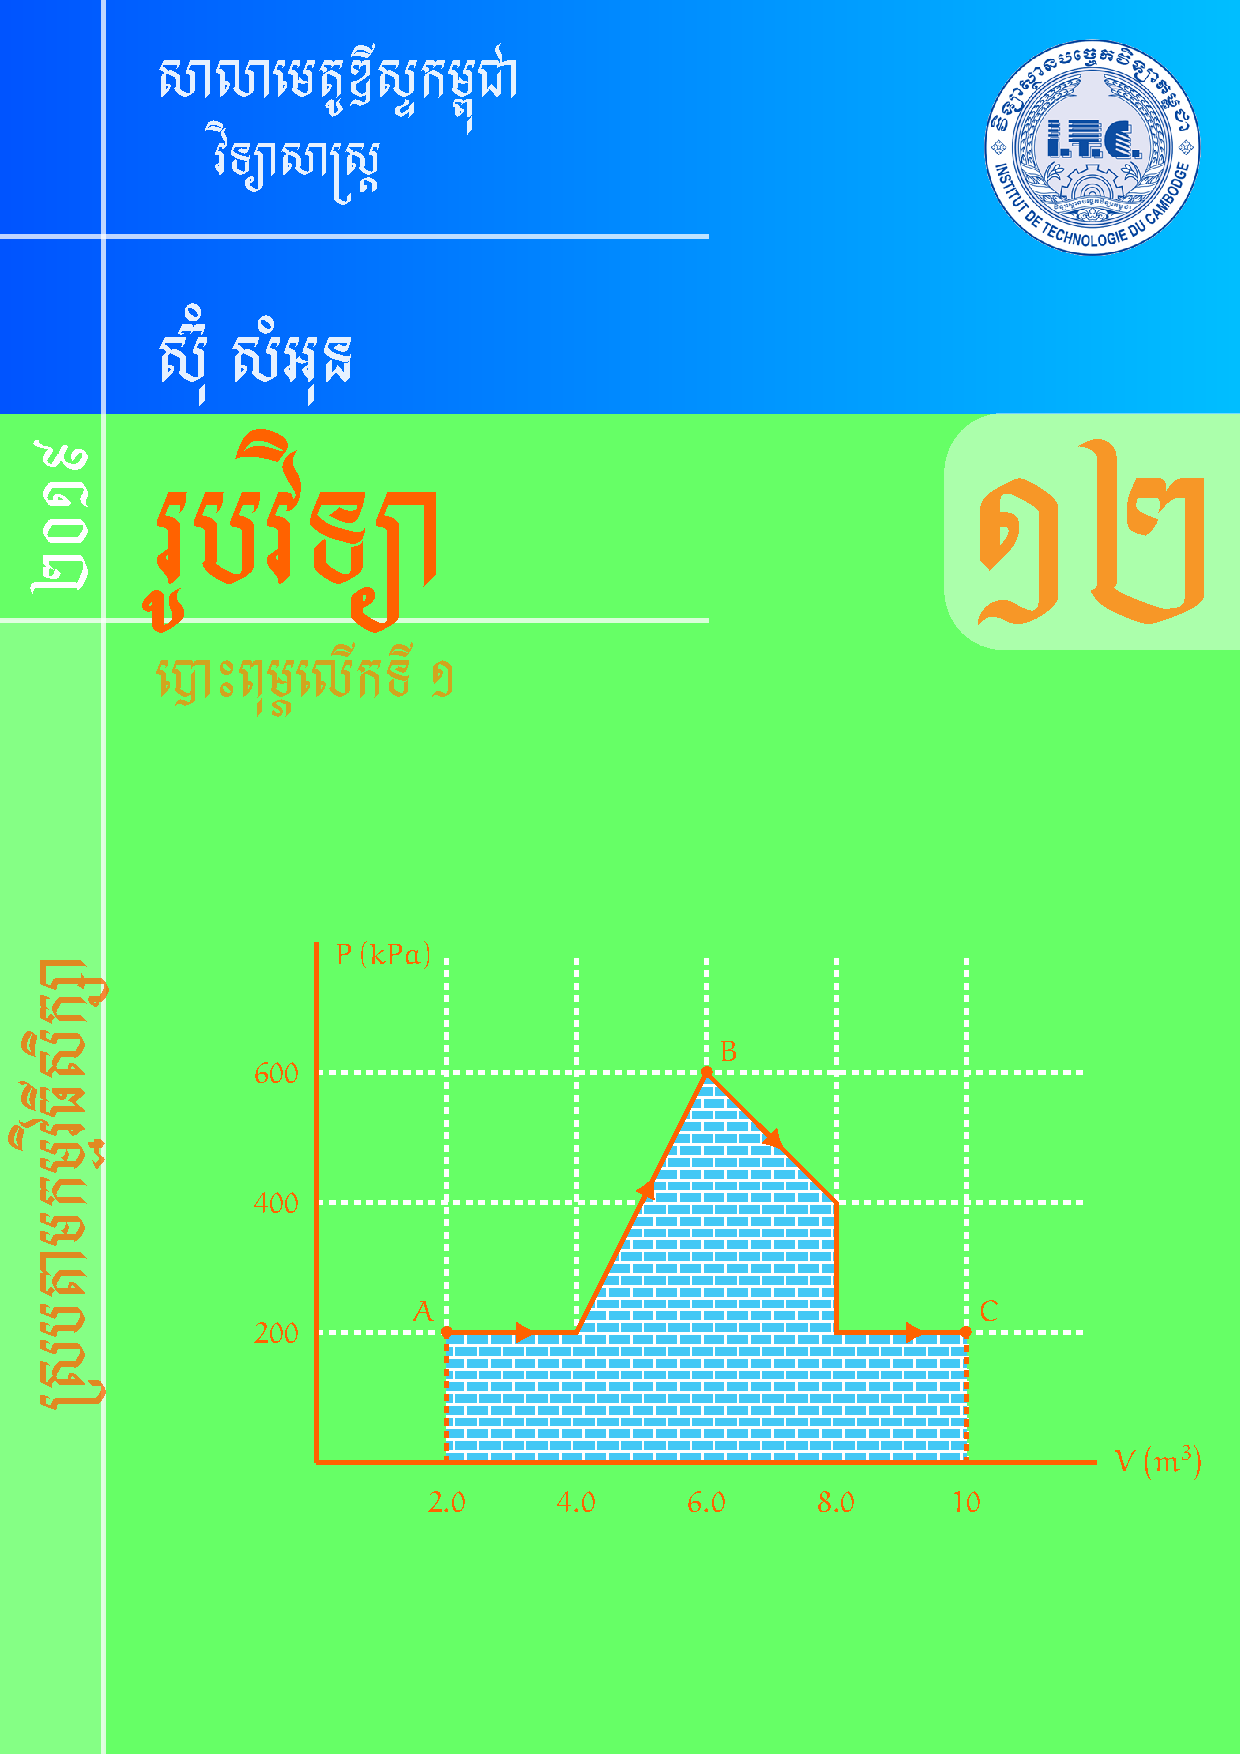
\includepdf[pages=1]{conicfrontcover.pdf}
	%\frontmatter
	\pagenumbering{alpkh}
	%\chapter*{សេចក្ដីថ្លែងអំណរគុណ}
\addcontentsline{toc}{chapter}{សេចក្ដីថ្លែងអំណរគុណ}
ខ្ញុំសូមថ្លែងអំណរគុណយ៉ាងជ្រាលជ្រៅដល់មាតាបិតារបស់ខ្ញុំគឺ លោកឪពុក \emph{ឌុច~ទាក់} និង អ្នកម្ដាយ \emph{ឌុក~សារុំ} ដែលបានផ្ដល់អ្វីគ្រប់យ៉ាងដល់រូបខ្ញុំ។ ខ្ញុំសូមថ្លែងអំណរគុណដល់ លោកពូ \emph{ស៊ិន~អ៊ាន} និង អ្នកមីង \emph{ឌុក~សាភូ} ដែលទំនុកបម្រុង ផ្ដល់ដំបូន្មាន និង ការជម្រុញលើកទឹកចិត្ត។ សូមផ្ញើរសេចក្ដីថ្លែងអំណរគុណដល់បងប្អូនខ្ញុំជាច្រើនអ្នកទៀត។
\\[1em]
ជាថ្មីម្ដងទៀតខ្ញុំសូមរំលឹកគុណដល់លោកគ្រូ អ្នកគ្រូរបស់ខ្ញុំដែលបាន បង្ហាត់ពត់លត់ដំខាងផ្នែកបញ្ញាស្មារតី និងវិជ្ជាជីវៈ។ បន្ថែមលើនេះខ្ញុំសូមថ្លែងអំណរគុណដល់មិត្តភ័ក្ដិ និងសិស្សានុសិស្សដែលបានផ្ដល់ជាកំលាំងចិត្តដល់រូបខ្ញុំ។
	%\chapter*{អារម្ភកថា}
\addcontentsline{toc}{chapter}{អារម្ភកថា}
កថាខណ្ឌនេះពិពណ៌នាអំពីដំណើរដងទងនៃការចាប់កំណើតឡើងនៃសៀវភៅនេះ។ ដំបូងឡើយវាគ្រាន់តែជាកម្រងលំហាត់សម្រាប់ឲ្យសិស្សអនុវត្តន៏បន្ថែមលើការសិក្សាម៉ោងរដ្ធតែប៉ុណ្ណោះ។ ដោយពេលវេលាមានរយៈពេលខ្លី ការដាក់ឧទាហរណ៏ និងលំហាត់គំរូពុំសូវបានច្រើនជាហេតុបណ្ដាលអោយខ្ញុំកើតគំនិតសរសេរចម្លើយដើម្បីអោយសិស្សអាន និងអនុវត្តន៏ដោយខ្លួនឯង។
\\[1em]
សៀវភៅនេះបែងចែកជាបួនផ្នែករួមមាន មេរៀនសង្ខេបអមដោយឧទាហរណ៏គំរូ កម្រងលំហាត់បញ្ចប់មេរៀន ចម្លើយលំហាត់ និង សេចក្ដីបន្ថែម។ នៅផ្នែកមេរៀនសង្ខេបយើងមាន ការរំលឹកខ្លី និយមន័យ លក្ខណៈ និងទ្រឹស្ដីបទ។ ឧទាហរណ៏គំរូសម្រាប់និយមន័យនីមួយៗ ក៏ត្រូវបានរួមបញ្ចូលនៅផ្នែកនេះដែរ។ សម្រាប់សម្រាយបញ្ជាក់ លក្ខណៈ និងទ្រីស្ដីបទសំខាន់អ្នកអានរកមើលនៅផ្នែកបន្ថែមដែលបានដាក់នៅជំពូកចុងក្រោយគេបង្អស់នៃសៀវភៅ។ នៅផ្នែកកម្រងលំហាត់បញ្ចប់មេរៀន យើងមានតែលំហាត់សុទ្ធដែលត្រូវបានរៀបចំតាមខ្លឹមសារមេរៀន និងតាមលំដាប់កើននៃភាពលំបាក។ បន្ទាប់ពីផ្នែកនេះគឺជាចម្លើយលើកម្រងលំហាត់។ រីឯផ្នែកចុងក្រោយ ជាសេចក្ដីបន្ថែម ដែលភាគច្រើនដកស្រង់ចេញពីមេរៀនថ្នាក់ក្រោម។ អ្នកអានគួរផ្ដោតការយកចិត្តទុកលើផ្នែកនេះជាចំបង។ ផ្នែកនេះគួរតែអានមុនគេដើម្បីបង្កភាពងាយស្រួលក្នុងការអានផ្នែកផ្សេងៗទៀត។
\\[1em]
បញ្ជាក់ជួនដល់អ្នកអានសៀវភៅនេះឲ្យបានជ្រាបថា វាគឺជាស្នារដៃដំបូងរបស់អ្នកនិពន្ធ។ សៀវភៅនេះត្រូវបានបង្កើតឡើងដោយមនុស្សតែម្នាក់ប៉ុណ្ណោះ។ ជាងនេះទៅទៀតវាពុំទាន់បានឆ្លងកាត់ការត្រួតពិនិត្យទាំងផ្នែកបច្ចេកទេស និងអក្ខរាវិរុទ នៅឡើយទេ។ បើប្រិយមិត្តរកឃើញកំហុសឆ្គងណាមួយ សូមជួនដំណឹងដល់អ្នកសរសេរសៀវភៅដោយការផ្ញើរសារជាអក្សរ ឬ រូបភាពមកកាន់ប្រអប់សារអេឡិចត្រូនិច ដែលមានអាស័យដ្ឋាន \textcolor{magenta}{\itshape bunnybookauthor@gmail.com} បើមិនអញ្ចឹងទេអ្នកអាចជួបពិភាក្សាផ្ទាល់បើអាចធ្វើទៅបាន។
\\[1em]
ទាក់ទិននឹងការធ្វើអាជីវកម្មលើសៀវភៅនេះ អ្នកនិពន្ធរក្សាសិទ្ធិកម្មសិទ្ធិបញ្ញាដោយមិនអនុញ្ញាតអោយធ្វើការបោះពុម្ភ ថតចំលង ឬចែកចាយដោយគ្មានការអនុញ្ញាតឡើយ។ ចំពោះកំណាត់សៀវភៅនេះជាឯកសារអេឡិចត្រូនិច អ្នកអាចទាញយកមកអាន និងប្រើប្រាស់ផ្ទាល់ខ្លួនបានដោយមិនគិតថ្លៃតាមរយៈដំណរ\\ \textcolor{magenta}{\itshape bunnybookshelf.blogspot.com/p/conic.html}~។
	%\clearpage
\tableofcontents
\addcontentsline{toc}{chapter}{\contentsname}
	%\mainmatter
	\pagenumbering{khmer}
	\chapter{មូលដ្ឋានគ្រឹះខ្លះៗនៃគណិតវិទ្យា}
\section{ស្វ័យគុណ}
\quad ស្វ័យគុណត្រូវបានប្រើជាញឹកញាប់នៅក្នុងរូបវិទ្យា ពេលយើងសរសេរ $3^{4}$ ដែល $4$ ហៅថាស្វ័យគុណ ហើយ $3$ ជាគោល។ យើងអាចអានបានថា $3$ ស្វ័យគុណ $4$។
\begin{formula}
	\begin{enumerate}[m,2]
		\item $a^{0}=1\quad \left(a\ne 0\right)$
		\item $a^{n}=a\times a\times a \times \cdots \times a\quad\left(a\ne 0\right)$
%		\emph{ឧទាហរណ៍ទី១ៈ} $10^{4}=10\times10\times10\times10=10000$\\
%		\emph{ឧទាហរណ៍ទី២ៈ} $10^{2}=10\times10=100$
		\item $a^{-n}=\frac{1}{a^{n}}\quad \left(a\ne 0\right)$
		\item $a^{m}\cdot a^{n}=a^{m+n}\quad \left(a\ne 0, n\ne 0, m\ne 0\right)$
		\item $\frac{a^{m}}{a^{n}}=a^{m-n}\quad \left(a\ne 0, n\ne 0, m\ne 0\right)$
		\item $\left(a\cdot b\right)^{n}=a^{n}\cdot b^{n}\quad \left(n\ne 0\right)$
		\item $\left(a^{m}\right)^{n}=\left(a^{n}\right)^{m}=a^{m\cdot n}\quad \left(a\ne 0, n\ne 0, m\ne 0\right)$
		\item $\left(\frac{a}{b}\right)^{n}=\frac{a^{n}}{b^{n}}\quad \left(b\ne 0, n\ne 0\right)$
	\end{enumerate}
\end{formula}
\section{ឯកលក្ខណៈភាពសំខាន់ៗ}
\begin{formula}
	\begin{enumerate}[m,2]
		\item $\left(a+b\right)^{2}=a^{2}+2ab+b^{2}$
		\item $\left(a-b\right)^{2}=a^{2}-2ab+b^{2}$
		\item $\left(a+b\right)^{3}=a^{3}+3a^{2}b+3ab^{2}+b^{3}$
		\item $\left(a+b\right)^{3}=a^{3}-3a^{2}b+3ab^{2}-b^{3}$
		\item $a^{2}-b^{2}=\left(a-b\right)\left(a-b\right)$
		\item $a^{2}+b^{2}=\left(a+b\right)^{2}-2ab$
		\item $a^{3}-b^{3}=\left(a-b\right)\left(a^{2}+ab+b^{2}\right)$
		\item $a^{3}+b^{3}=\left(a+b\right)\left(a^{2}-ab+b^{2}\right)$
	\end{enumerate}
\end{formula}
\section{លក្ខណៈនៃប្រភាគពីរស្មើគ្នា}
\begin{generality}
	ឧបមាថាយើងមានប្រភាគពីរស្មើគ្នា $\frac{a}{b}=\frac{c}{d}$។ យើងអាចសរសេរបានដូចខាងក្រោមៈ
	\begin{enumerate}[m,2]
		\item $\frac{d}{b}=\frac{c}{a}$ (ប្តូរតួចុង)
		\item $\frac{a}{c}=\frac{b}{d}$ (ប្តូរតួមធ្យម)
		\item $a\cdot d=b\cdot c$ (ផលគុណតួចុងស្មើនឹងផលគុណតួមធ្យម)
		\item $\frac{a}{b}=\frac{c}{d}=\frac{a\pm c}{b\pm d}$ (លក្ខណៈផលធៀបស្មើតគ្នា)
	\end{enumerate}
\end{generality}
\section{សមីការបន្ទាត់}
\begin{formula}
	សមីការបន្ទាត់មានរាង $y=ax+b$ ដែល $a$ ជាមេគុណប្រាប់ទិស និង $b$ ជាចំនួនថេរ។ បើ $b=0$ នោះសមីការបន្ទាត់មានរាង $y=ax$ គេថាបន្ទាត់កាត់តាមគល់ $0$។
	\begin{align*}
		\text{មេគុណប្រាប់ទិសនៃបន្ទាត់គឺ}\quad :&\quad a=\frac{\Delta y}{\Delta x}=\frac{y_{2}-y_{1}}{x_{2}-x_{1}}
	\end{align*}
\end{formula}
\section{ទម្រង់ស្តង់ដានៃស្វ័យគុណ}
 ទម្រង់ស្តង់ដានៃស្វ័យគុណរបស់ចំនួនមួយគឺជាផលគុណនៃចំនួន $A$ ដែល $1\le A<10$ នឹងស្វ័យគុណ $10$។ ដូចនេះទម្រង់ស្តង់ដាមានរាង $A\times10^{n}$ ដែល $1\le A<10$ ហើយ $n$ ជាចំនួនគត់រុឺឡាទីប។
 \begin{example}
 	សរសេរចំនួនខាងក្រោមជាទម្រង់ស្តង់ដាៈ
 	\begin{enumerate}[k,2]
 		\item $550~000~000=55\times10^{7}$
 		\item $0.000~000~343=343\times10^{-9}$
 		\item $0.000~000~000~004mm=4\times10^{-12}mm$
 		\item $300~000km/s=3\times10^{5}km/s$
 	\end{enumerate}
 \end{example}
\section{ទ្រឹស្តីបទកូសុីនុស និងសុីនុស}
\begin{theorem}
	\begin{multicols}{2}
		\emph{\kml $\bullet$ ទ្រឹស្តីបទកូសុីនុស}
		\begin{align*}
		a^{2}=b^{2}+b^{2}-2bc\cos\alpha\\
		b^{2}=a^{2}+c^{2}-2ac\cos\beta\\
		c^{2}=a^{2}+b^{2}-2ab\cos\gamma\\
		\end{align*}
		\emph{\kml $\bullet$ ទ្រឹស្តីបទសុីនុស}
		\begin{align*}
		\frac{a}{\sin \alpha}=\frac{b}{\sin \beta}=\frac{c}{\sin \gamma}=2R\\ \text{$R$ ជាកាំរង្វង់ចរឹកក្រៅត្រីកោណ}
		\end{align*}
		\emph{\kml $\bullet$ ផលបូកមុំក្នុងនៃត្រីកោណៈ} $\alpha + \beta + \gamma=180^\circ$
		\begin{figure}[H]
			\centering
			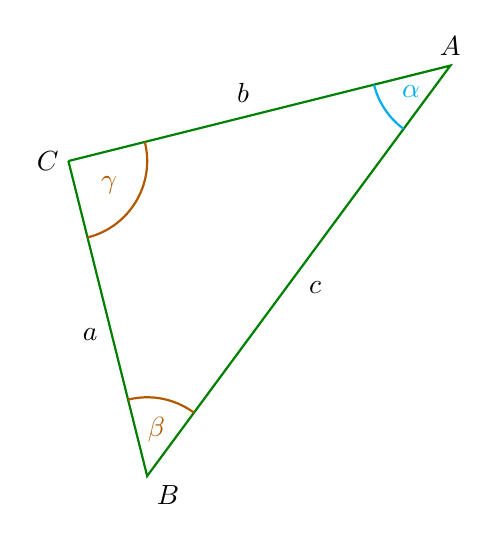
\begin{tikzpicture}[scale=1]
			\RectTri{(0,4)}{(1,0)}{5cm}
			\end{tikzpicture}
			\caption{ត្រីកោណនៃទ្រឹស្តីបទកូសុីនុស និងសុីនុស}
		\end{figure}
	\end{multicols}
\end{theorem}
\section{ផលគុណស្កាលែនៃពីរវុិចទ័រ}
	\begin{multicols}{2}
	\emph{\kml ផលគុណស្កាលែនៃពីរវុិចទ័រៈ} បើគេមានវុិចទ័រពីរ $\overrightarrow{A}$ និង $\overrightarrow{B}$ ដែលផ្គុំគ្នាបានមុំ $\theta$ ដូចរូបខាងស្តាំ។ \newline
	នោះគេអាចសរសេរ
		\begin{align*}
			\text{គេសរសេរ}\quad :&\quad\overrightarrow{A}\cdot\overrightarrow{B}=\abs{\overrightarrow{A}}\abs{\overrightarrow{B}}\cos\theta\\
			\text{ម្យ៉ាងទៀត}\quad :&\quad \quad\overrightarrow{A}\cdot\overrightarrow{B}=AB\cos\theta
		\end{align*}
		\begin{figure}[H]
			\centering
			\begin{tikzpicture}
			\begin{scope}
			\coordinate (O) at (0,0);
			\coordinate (A) at (2,2);
			\coordinate (B) at (3,0);
			\coordinate (C) at (4,2);
			\draw [->] (O) -- (A);
			\draw [->] (O) -- (B);
			\draw [dashed] (A) -- (2,0);
			\coordinate[label=above:$\overrightarrow{A}$] (A) at (A);
			\coordinate[label=below:$\overrightarrow{B}$] (B) at (B);
			\pic [draw, -, "$\theta$", angle eccentricity=1.5] {angle = B--O--A};
			\end{scope}
			\end{tikzpicture}
			\caption{\koc ផលគុណស្កាលែនៃពីរវុិចទ័រ}
		\end{figure}
	\end{multicols}
\section{ធរណីមាត្រក្នុងប្លង់ និងអនុគមន៍ត្រីកោណមាត្រ}
\subsection{ការេ}
	\chapter{ទំហំវុិចទ័រ និងទំហំស្កាលែ}
\section{ទំហំវុិចទ័រ}
\subsection{ទំហំវិុចទ័រ}
\begin{definition}
	\emph{{\kml ទំហំវិុចទ័រៈ}} ជាទំហំដែលសំដែងជាតម្លៃពីជគណិត ហើយអាស្រ័យនឹង ទិស ទិសដៅ។ វុិចទ័រមួយជាអង្គត់ដែលមានទិសដៅ ភ្ជាប់ពីរចំណុចផ្សេងគ្នា ដែលចំណុចំណុចមួយជាគល់ ឬចំណុចចាប់ និងមួយទៀតជាចុងនៃវុិចទ័រ។
\end{definition}
\begin{example}
	ទំហំវិុចទ័ររួមមានៈ កម្លាំង ល្បឿន សំទុះទំនាញដី ដែនម៉ាញេទិច។ ល។ យើងអាចលើកយកវុិចទ័រ $\overrightarrow{OA}$ មកសិក្សាៈ
	\begin{multicols}{2}
		\begin{itemize}
			\item [$-$] ចំណុចចាប់ ឬគល់ៈ ត្រង់ $O$
			\item [$-$] ទិសៈ ស្ថិតលើបន្ទាត់ $OA$
			\item [$-$] ទិសដៅពី $O$ ទៅ $A$(សម្គាល់ដោយព្រួញ)
			\item [$-$] អាំងតង់សុីតេ ឬម៉ូឌុលៈ $\abs{\overrightarrow{OA}}$
		\end{itemize}
		\begin{figure}[H]
			\centering
			\begin{tikzpicture}[scale=1]
				\begin{scope}
					\coordinate (O) at (0,0);
					\coordinate (A) at (3,2);
					\draw [->] (O) -- (A);
					\coordinate [label=below:$O$] (O) at (O);
					\coordinate [label=above:$A$] (A) at (A);
					\draw (O) node {$\bullet$};
					\draw (1.2,1.5) node {$\overrightarrow{OA}$};
				\end{scope}
			\end{tikzpicture}
			\caption{វុិចទ័រ}
		\end{figure}
	\end{multicols}
\end{example}
\subsection{វុិចទ័រពីរស្មើគ្នា}
\begin{definition}
	\emph{{\kml វុិចទ័រពីរស្មើគ្នាៈ}} កាលណាវុិចទ័រទាំងពីរនោះមានប្រវែងស្មើគ្នា និងមានទិសដៅដូចគ្នា។
\end{definition}
\begin{example}
	ចូរពិនិត្យមើលវិុចទ័រ $\overrightarrow{A}$ និង $\overrightarrow{B}$ ដូចរូបខាងក្រោម។ យើងឃើញថាវុិចទ័រទាំងពីរនេះមានម៉ូឌុល ឬប្រវែងស្មើគ្នា និងមានទិសដៅដូចគ្នា។
	\begin{figure}[H]
		\centering
		\begin{tikzpicture}
			\begin{scope}
				\draw[->] (.1,-.8) --(6,-.8);
				\draw[->] (.5,-1.2) --(.5,2.5);
				\coordinate (O) at (0,0);
				\coordinate (A) at (3,2);
				\coordinate (B) at (2,0);
				\coordinate (C) at (5,2);
				\draw [->] (O) -- (A);
				\draw [->] (B) -- (C);
				\draw (1.2,1.5) node {$\overrightarrow{A}$};
				\draw (3.2,1.5) node {$\overrightarrow{B}$};
				\coordinate [label=below:$O$] (O) at (0.2,-.8);
				\coordinate [label=left:$y$] (y) at (0.5,2.2);
				\coordinate [label=below:$x$] (x) at (6,-.8);
			\end{scope}
		\end{tikzpicture}
		\caption{វុិចទ័រពីរស្មើគ្នា}
	\end{figure}
	ដូចនេះ វុិចទ័រ $\overrightarrow{A}$ ស្មើនឹង $\overrightarrow{B}$ ឬវុិចទ័រទាំងពីរនេះសមភាពគ្នា ទោះបីវាចេញពីគល់ផ្សេងគ្នាក៏ដោយ។ 
	\begin{align*}
		\text{គេសរសេរៈ}\quad :&\quad \overrightarrow{A}=\overrightarrow{B}\\
		\text{នាំឲ្យ}​\quad :&\quad \abs{\overrightarrow{A}}=\abs{\overrightarrow{B}}\quad \text{ឬ}\quad A=B
	\end{align*}
\end{example}
\subsection{ផលបូកវុិចទ័រ}
\begin{enumerate}[m]
	\item \emph{\kml ផលបូកវុិចទ័រពីរមានទិស និងទិសដៅដូចគ្នា}
	\begin{multicols}{2}
			\quad គេមានវុិចទ័រពីរ $\overrightarrow{A}$ និង $\overrightarrow{B}$ ដូចរូបខាងស្តាំ។\\
		យើងបានវិុចទ័រផ្គួបនៃវុិចទ័រ $\overrightarrow{A}$ និង $\overrightarrow{B}$ គឺ $\fbox{$\overrightarrow{C}=\overrightarrow{A}+\overrightarrow{B}$}$
		\begin{figure}[H]
			\centering
			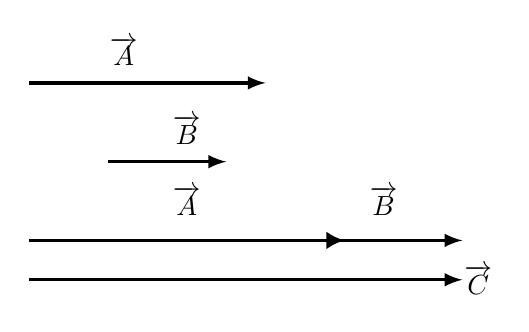
\begin{tikzpicture}
			\begin{scope}[very thick, every node/.style={sloped,allow upside down}]
			\coordinate (O) at (0,2);
			\coordinate (A) at (3,2);
			\coordinate (B) at (1,1);
			\coordinate (C) at (2.5,1);
			\coordinate (D) at (5.5,0);
			\draw [->] (O) -- (A);
			\draw [->] (B) -- (C);
			\draw [->] (0,0) -- (D);
			\draw [arrows = {-Latex[width=6.5pt, length=6.5pt]}] (3.8,0) -- (4,0);
			\draw (1.2,2.4) node {$\overrightarrow{A}$};
			\draw (2,1.4) node {$\overrightarrow{B}$};
			\draw (2,.5) node {$\overrightarrow{A}$};
			\draw (4.5,.5) node {$\overrightarrow{B}$};
			\draw [->] (0,-.5) -- (5.5,-.5);
			\draw (5.7,-.5) node {$\overrightarrow{C}$};
			\end{scope}
			\end{tikzpicture}
			\caption{ផលបូកវុិចទ័រពីរមានទិស និងទិសដៅដូចគ្នា}
		\end{figure}
	\end{multicols}
	ក្នុងករណីដែលយើងចង់រកម៉ូឌុលនៃវុិច $\overrightarrow{C}$ យើងត្រូវលើកអង្គទាំងពីរជាការេ
	\begin{align*}
		\text{យើងបាន}\quad :&\quad \overrightarrow{C^{2}} =\left(\overrightarrow{A}+\overrightarrow{B}\right)^{2}=\overrightarrow{A^{2}} + 2\overrightarrow{A}\overrightarrow{B}+\overrightarrow{B^{2}}=\overrightarrow{A^{2}} + 2AB\cos\left(\overrightarrow{A},\overrightarrow{B}\right) +\overrightarrow{B^{2}}\\
		\text{ដោយ}\quad :&\quad \overrightarrow{C^{2}}=C^{2},~\overrightarrow{A^{2}}=A^{2},~\overrightarrow{B^{2}}=B^{2},~\left(\overrightarrow{A},\overrightarrow{B}\right)=0\\
		\text{យើងបាន}\quad :&\quad C^{2}=A^{2}+2AB+B^{2}=\left(A+B\right)^{2}\\
		\text{នាំឲ្យ}\quad :&\quad C=\sqrt{\left(A+B\right)^{2}}=A+B
	\end{align*}
	\begin{generality}
		អាំងតង់សុីតេវុិចទ័រផ្គួបដែលមានទិសស្របគ្នា និងទិសដៅដូចគ្នាស្មើនឹងផលបូកអាំងតង់សុីតេនៃវុិចទ័រផ្គុំទាំងអស់។
	\end{generality}
	\item \emph{\kml ផលបូកវុិចទ័រពីរមានទិសដូចគ្នា និងទិសដៅផ្ទុយគ្នា}
	\begin{multicols}{2}
		គេមានវុិចទ័រពីរ $\overrightarrow{A}$ និង $\overrightarrow{B}$ ដូចរូបខាងស្តាំ។ គេបានវុិចទ័រ $\overrightarrow{C}=\overrightarrow{A}+\left(-\overrightarrow{B}\right)=\overrightarrow{A}-\overrightarrow{B}\Rightarrow\fbox{$C=A-B$}$\\
		\begin{figure}[H]
			\centering
			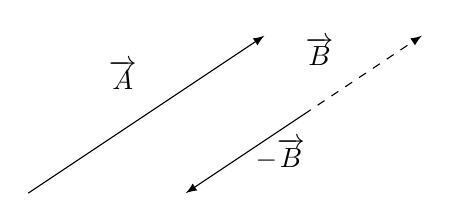
\begin{tikzpicture}
			\begin{scope}
			\coordinate (O) at (0,0);
			\coordinate (A) at (3,2);
			\coordinate (B) at (2,0);
			\coordinate (C) at (3.5,1);
			\coordinate (D) at (3.5,1);
			\coordinate (E) at (5,2);
			\draw [->] (O) -- (A);
			\draw [<-] (B) -- (C);
			\draw[->, dashed] (D) -- (E);
			\draw (1.2,1.5) node {$\overrightarrow{A}$};
			\draw (3.7,1.8) node {$\overrightarrow{B}$};
			\draw (3.2,.5) node {$-\overrightarrow{B}$};
			\end{scope}
			\end{tikzpicture}
			\caption{វុិចទ័រពីរមានទិសដូចគ្នា និងទិសដៅផ្ទុយគ្នា}
		\end{figure}
	\end{multicols}
	\begin{multicols}{2}
		ដើម្បីសង់វុិចទ័រផ្គួប $\overrightarrow{C}$ យើងរំកិលវុិចទ័រ $\overrightarrow{B}$ ដោយរក្សាទិសរបស់វាទៅដាក់លើទិសនៃវុិចទ័រ $\overrightarrow{A}$ ដោយដាក់គល់នៃវុិចទ័រ $\overrightarrow{B}$ លើចុងស្លាបព្រួញនៃវុិចទ័រ $\overrightarrow{A}$។
		\begin{figure}[H]
			\centering
			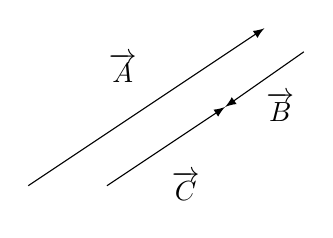
\begin{tikzpicture}
			\begin{scope}
			\coordinate (O) at (0,0);
			\coordinate (A) at (3,2);
			\coordinate (B) at (1,0);
			\coordinate (C) at (2.5,1);
			\coordinate (D) at (2.5,1);
			\coordinate (E) at (3.5,1.7);
			\draw [->] (O) -- (A);
			\draw [->] (B) -- (C);
			\draw[<-] (D) -- (E);
			\draw (1.2,1.5) node {$\overrightarrow{A}$};
			\draw (3.2,1) node {$\overrightarrow{B}$};
			\draw (2,0) node {$\overrightarrow{C}$};
			\end{scope}
			\end{tikzpicture}
			\caption{\DS ផលបូកវុិចទ័រពីរមានទិសដូចគ្នា និងទិសដៅផ្ទុយគ្នា}
		\end{figure}
	\end{multicols}	
	\begin{remark}
		ទិសដៅនៃវុិចទ័រផ្គួបគឺដូចនឹងទិសដៅនៃវុិចទ័រដែលមានអាំងតង់សុីតេធំជាងគេ។
	\end{remark}
	\item \emph{\kml ផលបូកវុិចទ័រពីរមានទិសបង្កើតបានមុំ $\theta$}
		\begin{multicols}{2}
			\quad គេមានវុិចទ័រពីរ $\overrightarrow{A}$ និង $\overrightarrow{B}$ ដែលផ្គុំគ្នាបានមុំ $\theta$ ដូចរូបខាងស្តាំ។ យើងបានវុិចទ័រផ្គួបនៃវុិចទ័រ $\overrightarrow{A}$ និង $\overrightarrow{B}$ គឺតាងដោយ $\overrightarrow{C}=\overrightarrow{A}+\overrightarrow{B}$
			\begin{figure}[H]
				\centering
				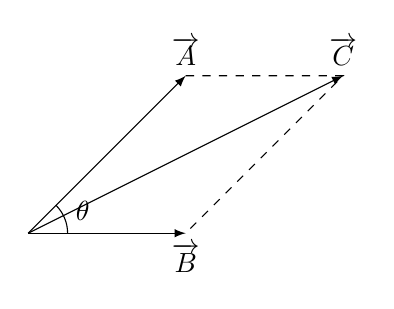
\begin{tikzpicture}
				\begin{scope}
				\coordinate (O) at (0,0);
				\coordinate (A) at (2,2);
				\coordinate (B) at (2,0);
				\coordinate (C) at (4,2);
				\draw [->] (O) -- (A);
				\draw [->] (O) -- (B);
				\draw [->] (O) -- (C);
				\draw [dashed] (2,2) --(4,2) -- (2,0);
				\coordinate[label=above:$\overrightarrow{A}$] (A) at (A);
				\coordinate[label=below:$\overrightarrow{B}$] (B) at (B);
				\coordinate[label=above:$\overrightarrow{C}$] (C) at (C);
				\pic [draw, -, "$\theta$", angle eccentricity=1.5] {angle = B--O--A};
				\end{scope}
				\end{tikzpicture}
				\caption{ផលបូកវុិចទ័រពីរមានទិសបង្កើតបានមុំ $\theta$}
			\end{figure}
		\end{multicols}
		យើងអាចលើកអង្គទាំងពីរនៃសមីការនេះជាការេ
		\begin{align*}
		\text{យើងបាន}\quad :&\quad \overrightarrow{C^{2}} =\left(\overrightarrow{A}+\overrightarrow{B}\right)^{2}=\overrightarrow{A^{2}} + 2\overrightarrow{A}\overrightarrow{B}+\overrightarrow{B^{2}}=\overrightarrow{A^{2}} + 2AB\cos\left(\overrightarrow{A},\overrightarrow{B}\right) +\overrightarrow{B^{2}}\\
		\text{ដោយ}\quad :&\quad \overrightarrow{C^{2}}=C^{2},~\overrightarrow{A^{2}}=A^{2},~\overrightarrow{B^{2}}=B^{2},~\left(\overrightarrow{A},\overrightarrow{B}\right)=\theta\\
		\text{យើងបាន}\quad :&\quad C^{2}=A^{2}+B^{2} + 2AB\cos\theta\\
		\text{នាំឲ្យ}\quad :&\quad C=\sqrt{A^{2}+B^{2}+2AB\cos\theta}
		\end{align*}
	\begin{remark}
		ដើម្បីសង់វុិចទ័រផ្គួប $\overrightarrow{C}$ ដែល $\overrightarrow{C}=\overrightarrow{A}+\overrightarrow{B}$ យើងត្រូវអនុវត្តតាមវិធានអង្តត់ទ្រូងប្រលេឡូក្រាម។
	\end{remark}
	\item \emph{\kml ផលបូកវុិចទ័រពីរមានទិស និងទិសដៅកែងគ្នា}
	\begin{multicols}{2}
		\quad គេមានវុិចទ័រពីរ $\overrightarrow{A}$ និង $\overrightarrow{B}$ ដែលផ្គុំគ្នាបានមុំ $90^\circ$ ឬមានទិស និងទិសដៅកែងគ្នា ដូចរូបខាងស្តាំ។ យើងបានវុិចទ័រផ្គួបនៃវុិចទ័រ $\overrightarrow{A}$ និង $\overrightarrow{B}$ គឺតាងដោយ $\overrightarrow{C}=\overrightarrow{A}+\overrightarrow{B}$
		\begin{figure}[H]
			\centering
			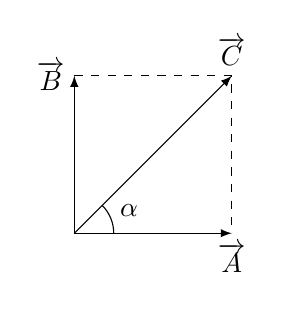
\begin{tikzpicture}
			\begin{scope}
			\coordinate (O) at (0,0);
			\coordinate (A) at (2,0);
			\coordinate (B) at (0,2);
			\coordinate (C) at (2,2);
			\draw [->] (O) -- (A);
			\draw [->] (O) -- (B);
			\draw [->] (O) -- (C);
			\draw [dashed] (0,2) --(2,2) -- (2,0);
			\coordinate[label=below:$\overrightarrow{A}$] (A) at (A);
			\coordinate[label=left:$\overrightarrow{B}$] (B) at (B);
			\coordinate[label=above:$\overrightarrow{C}$] (C) at (C);
			\pic [draw, -, "$\alpha$", angle eccentricity=1.5] {angle = A--O--C};
			\end{scope}
			\end{tikzpicture}
			\caption{\DS ផលបូកវុិចទ័រពីរមានទិស និងទិសដៅកែងគ្នា}
		\end{figure}
	\end{multicols}
	យើងអាចលើកអង្គទាំងពីរនៃសមីការនេះជាការេ
	\begin{align*}
		\text{យើងបាន}\quad :&\quad \overrightarrow{C^{2}} =\left(\overrightarrow{A}+\overrightarrow{B}\right)^{2}=\overrightarrow{A^{2}} + 2\overrightarrow{A}\overrightarrow{B}+\overrightarrow{B^{2}}=\overrightarrow{A^{2}} + 2AB\cos\left(\overrightarrow{A},\overrightarrow{B}\right) +\overrightarrow{B^{2}}\\
		\text{ដោយ}\quad :&\quad \overrightarrow{C^{2}}=C^{2},~\overrightarrow{A^{2}}=A^{2},~\overrightarrow{B^{2}}=B^{2},~\left(\overrightarrow{A},\overrightarrow{B}\right)=90^\circ\\
		\text{យើងបាន}\quad :&\quad C^{2}=A^{2}+B^{2}\\
		\text{នាំឲ្យ}\quad :&\quad C=\sqrt{A^{2}+B^{2}}
	\end{align*}
\end{enumerate}
\section{ទំហំស្កាលែ}
\begin{definition}
	\emph{\kml ទំហំស្កាលែៈ} គឺជាបរិមាណចំនួន ឬទំហំក្នុងខ្នាតសមស្របមួយដែលគ្មានទិសដៅ។ នៅក្នុងរូបវិទ្យាទំហំដែលមិនទាក់ទងនឹងទិសដៅ(ទំហំស្កាលែ) មានដូចជាៈ សីតុណ្ហភាព សម្ពាធ ថាមពល កម្មន្ត ម៉ាស រយៈពេល។ ល។
\end{definition}
\section{កូអរដោនេនៃវិុចទ័រ}
	\begin{multicols}{2}
		ឧបមាថាយើងមានត្រីកោណកែង $ABC$ ដូចបង្ហាញក្នុងរូបខាងស្តាំ ។
		\begin{equation*}
			\sin\theta=\frac{\text{ជ្រុងឈម}}{\text{អុីប៉ូតេនុស}},\quad \cos\theta=\frac{\text{ជ្រុងជាប់}}{\text{អុីប៉ូតេនុស}},\quad \tan\theta=\frac{\text{ជ្រុងឈម}}{\text{ជ្រុងជាប់}}
		\end{equation*}
		\begin{figure}[H]
			\centering
			\begin{tikzpicture}
				\centering 
				\begin{scope}
				\large
				\coordinate (C) at (0,0);
				\coordinate (A) at (3,0);
				\coordinate (B) at (3,2);
				\draw (C) -- (A) -- (B) -- cycle;
				\pic [draw, -, "$\theta$", angle eccentricity=1.5] {angle = A--C--B};
				\draw (A) -- ++ (0, .3cm) -- ++ (-.3cm, 0) -- ++ (0, -.3cm);
				\coordinate[label=below:$A$] (A) at (A);
				\coordinate[label=above:$B$] (B) at (B);
				\coordinate[label=below:$C$] (C) at (C);
				\coordinate[label=below:{\text{ជ្រុងជាប់}}] (1.5,0) at (1.5,0);
				\coordinate[label=right:{\text{ជ្រុងឈម}}] (3,1) at (3,1);
				\coordinate[label=right:{\text{អុីប៉ូតេនុស}}] (-1,1) at (-1,1);
				\end{scope}
			\end{tikzpicture}
			\caption{ទំនាក់ទំនងក្នុងត្រីកោណមាត្រ}
		\end{figure}
	\end{multicols}
	ទំនាក់ទំនង់រវាង $\sin\theta$ និង $\cos\theta$ គឺ
	\begin{align*}
		\tan\theta=\frac{\sin\theta}{\cos\theta} \quad \text{និង}\quad \sin^{2}\theta+\cos^{2}\theta=1
	\end{align*}
	\begin{multicols}{2}
		គេមានវុិចទ័រ $\overrightarrow{A}$ ស្តិតក្នុងប្លង់ $xy$ និងបង្កើតបានមុំ $\theta$ ជាមួយអ័ក្ស $Ox$ ដូចរូប។\\ យើងចំណោលកែងវុិចទ័រ $\overrightarrow{A}$ លើអ័ក្ស $Ox$ និង $Oy$ យើងបានធាតុរបស់វា{\en(Components of Vectors)}គឺ $\overrightarrow{A_{x}}$ និង $\overrightarrow{A_{y}}$។ តាមលក្ខណៈនៃវុិចទ័រយើងបានៈ $\overrightarrow{A}=\overrightarrow{A_{x}}+\overrightarrow{A_{y}}$
		\begin{figure}[H]
			\centering
			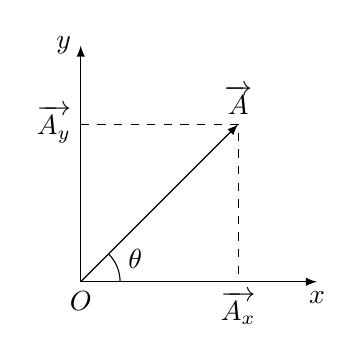
\begin{tikzpicture}
			\begin{scope}
			\coordinate (O) at (0,0);
			\coordinate (x) at (3,0);
			\coordinate (y) at (0,3);
			\coordinate (A) at (2,2);
			\draw [->] (O) -- (x);
			\draw [->] (O) -- (y);
			\draw [->] (O) -- (A);
			\draw [dashed] (0,2) --(2,2) -- (2,0);
			\coordinate[label=below:$x$] (x) at (x);
			\coordinate[label=left:$y$] (y) at (y);
			\coordinate[label=above:$\overrightarrow{A}$] (A) at (A);
			\coordinate[label=below:$\overrightarrow{A_{x}}$] (2,0) at (2,0);
			\coordinate[label=left:$\overrightarrow{A_{y}}$] (0,2) at (0,2);
			\coordinate[label=below:$O$] (0,0) at (0,0);
			\pic [draw, -, "$\theta$", angle eccentricity=1.5] {angle = x--O--A};
			\end{scope}
			\end{tikzpicture}
			\caption{ផលបូកវុិចទ័រពីរមានទិស និងទិសដៅកែងគ្នា}
		\end{figure}
	\end{multicols}
	\begin{proof}
		\begin{align*}
			\text{ដែល}\quad :&\quad A_{x}=A\cos\theta \quad\text{និង}\quad A_{y}=A\sin\theta\\
				\text{យើងបាន}\quad :&\quad \overrightarrow{A^{2}} =\left(\overrightarrow{A_{x}}+\overrightarrow{A_{y}}\right)^{2}=\overrightarrow{A^{2}_{x}} + 2\overrightarrow{A_{x}}\overrightarrow{A_{y}}+\overrightarrow{A_{y}^{2}}=\overrightarrow{A៌_{x}^{2}} + 2A_{x}A_{y}\cos\left(\overrightarrow{A_{x}},\overrightarrow{A_{y}}\right) +\overrightarrow{A_{y}^{2}}\\
			\text{ដោយ}\quad :&\quad \overrightarrow{A^{2}}=A^{2},~\overrightarrow{A_{x}^{2}}=A_{x}^{2},~\overrightarrow{A_{y}^{2}}=A_{y}^{2},~\left(\overrightarrow{A_{x}},\overrightarrow{A_{y}}\right)=90^\circ\\
			\text{យើងបាន}\quad :&\quad A^{2}=A_{x}^{2}+A_{y}^{2}\\
			\text{នាំឲ្យ}\quad :&\quad A=\sqrt{A_{x}^{2}+A_{y}^{2}}
		\end{align*}
	\end{proof}
	\chapter{ចលនាអង្គធាតុតាមមួយវិមាត្រ}
\section{ចលនាមេកានិច}
\begin{definition}
	\begin{itemize}
		\item បម្លាស់ប្តូរទីតាំងអង្គធាតុមួយធៀបនឹងអង្គធាតុមួយទៀត ហៅថាចលនាមេកានិច។
		\item ចំពោះអង្គធាតុណាមួយដែលកំណត់ចលនានៃអង្គធាតុផ្សេងទៀតធៀបនឹងវា គេហៅថាអង្គធាតុនោះថា តម្រុយ។
	\end{itemize}
\end{definition}
\section{បម្លាស់ទី ល្បឿន វុិចទ័រល្បឿន}
\subsection{ចម្ងាយចរ និងបម្លាស់ទី}
\begin{definition}
	\emph{\kml ចម្ងាយចរៈ} ជាប្រវែងសរុបនៃចលនារបស់អង្គធាតុដោយមិនគិតពីទិសដៅនៃចលនា។\\
	\emph{\kml បម្លាស់ទីៈ} ជាចម្ងាយចរដែលវាស់តាមខ្សែត្រង់ និងតាមទិសដៅជាក់លាក់។
\end{definition}
\begin{remark}
	លក្ខណៈសម្គាល់ទាំងពីរនៃបម្លាស់ទីគឺៈ
	\begin{itemize}
		\item [$-$] \emph{បម្លាស់ទី} គឺជាចម្ងាយចររវាងទីតាំងដើម និងទីតាំងស្រេចរបស់អង្គធាតុ។
		\item [$-$] \emph{បម្លាស់ទី} មានទិសដៅពីទីតាំងដើម​ទៅទីតាំងស្រេចរបស់អង្គធាតុ។
	\end{itemize}
\end{remark}
\subsection{ល្បឿន វុិចទ័រល្បឿន}
\begin{enumerate}[m]
	\item \emph{\kml ល្បឿន}\\
	ល្បឿននៃអង្គធាតុមួយសម្គាល់ភាពលឿន ឬភាពយឺតនៃចលនារបស់អង្គធាតុនោះ ហើយកំណត់ដោយផលធៀបរវាងចម្ងាយចរ និងរយៈពេល។ យើងបានៈ \fbox{$\text{ល្បឿន}=\frac{\text{ចម្ងាយចរ}}{\text{រយៈពេល}}$ ឬ $v=\frac{d}{t}$}\\
	\begin{multicols}{2}
		\begin{itemize}
			\item [$-$] ចម្ងាយចរគិតជាម៉ែត្រ $\left(m\right)$
			\item [$-$] រយៈពេលគិតជាវិនាទី $\left(s\right)$
			\item [$-$] ល្បឿនគិតជាម៉ែត្រក្នុងមួយវិនាទី $\left(m/s\right)$
		\end{itemize}
	\end{multicols}
	ភាកច្រើននៃអង្គធាតុមិនមានចលនាដោយល្បឿនថេរទេ ល្បឿនបស់វាពេលខ្លះយឺត និងពេលខ្លះលឿន។ ហេតុនេះហើយគេត្រូវកំណត់ល្បឿនរបស់អង្គធាតុនោះជាល្បឿនមធ្យមដែលល្បឿននេះដោយផលធៀបរវាងចម្ងាយចរសរុប និងរយៈពេលសរុប។\\
	យើងបានៈ \fbox{$\text{ល្បឿនមធ្យម}=\frac{\text{ចម្ងាយចរសរុប}}{\text{រយៈពេលសរុប}}$ ឬ $\overline{v}=\frac{d}{t}$}
	\item \emph{\kml វុិចទ័រល្បឿន}\\
	វុិចទ័រល្បឿនគឺជាបម្លាស់ទីរបស់វត្ថុក្នុងមួយខ្នាតពេល។\\
	យើងបានៈ \fbox{$\text{វុិចទ័រល្បឿន}=\frac{\text{បម្លាស់ទី(ចម្ងាយត្រង់)}}{\text{រយៈពេលចរ}}$}។
	\begin{multicols}{2}
		ឧបមាថានៅខណៈ $t_{1}$ ចល័តស្ថិតនៅត្រង់ចំណុចមួយដែលមានទីតាំង $x_{1}$ ហើយនៅខណៈ $t_{2}$ ចល័តស្ថិតនៅត្រង់ចំណុចមួយដែលមានទីតាំង $x_{2}$។
		\begin{figure}[H]
			\centering
			\begin{tikzpicture}
				\begin{scope}
					\draw [->, -Stealth] (-1,0) --(5,0);
					\coordinate[label=below:$O$] (0,0) at (0,0);
					\coordinate[label=below:$x_{1}$] (1,0) at (1,0);
					\coordinate[label=below:$x_{2}$] (3,0) at (3,0);
					\coordinate[label=above:$t_{1}$] (1,0) at (1,0);
					\coordinate[label=above:$t_{2}$] (3,0) at (3,0);
					\draw (0,0) node {$\bullet$};
					\draw (1,0) node {$\bullet$};
					\draw (3,0) node {$\bullet$};
					\draw [|-|] (1,1) --(3,1);
					\draw (2,1.5) node {$\Delta x$};
				\end{scope}
			\end{tikzpicture}
		\end{figure}
	\end{multicols}
	យើងបានៈ \fbox{$\text{វុិចទ័រល្បឿនមធ្យម}=\frac{\text{បម្លាស់ទីសរុប}}{\text{រយៈពេលចរ}}$ ឬ $v=\frac{\Delta x}{\Delta t}=\frac{x_{2}-x_{1}}{t_{2}-t_{1}}$}\\
	\quad នៅក្នុងជីវភាពរស់នៅយើងតែងតែប្រើពាក្យល្បឿនតែមួយគត់។ ប៉ូន្តែនៅក្នុងរូបវិទ្យា គេបានញែកពាក្យនេះជាពីរដាច់ចេញពីគ្នាគឺ ល្បឿន និង វុិចទ៏័រល្បឿន។ ល្បឿន ជាចម្ងាយចរក្នុងមួខ្នាតពេល។ ចំណែកឯវុិចទ័រល្បឿន ជាបម្លាស់ទីក្នុងមួយខ្នាតពេល។
	\begin{remark}
		កាលណាគេនិយាយពីវុិចទ័រល្បឿននៃអង្គធាតុមួយគេត្រូវគិតដល់ល្បឿននិងទិសដៅដែលវាបានឆ្លងកាត់។\\
		ក្នុងចលនាត្រង់ស្មើ វុិចទ័រល្បឿននិងវុិចទ័របម្លាស់ទីមានទិស និងទិសដៅដូចគ្នា ដូចនេះគេអាចសរសេរៈ $v=\frac{\Delta x}{\Delta t}$
	\end{remark}
\end{enumerate}
\subsection{វុិចទ័រល្បឿនខណៈ}


	%\chapter{ច្បាប់ចលនារបស់ញូតុន}
%\begin{objectives}
%\end{objectives}
\begin{introduction}
	\quad យើងបានសិក្សារួចមកហើយនៅមេរៀនមុនអំពី ល្បឿន សំទុះនៃចលនារបស់អង្គធាតុដោយយើងមិនបានគិត ឬពិនិត្យអំពីថាហេតុអ្វីដែលធ្វើឲ្យវាមានចលនាឡើយ(ផ្នែកស៊ីនេម៉ាទិច)។ ដោយលែកក្នុងមេរៀននេះយើងនឹងពិនិត្យមើលពីបុព្វហេតុដែលធ្វើឲ្យវត្ថុ ឬអង្គធាតុមួយមានចលនា(ផ្នែកឌីណាមិច)។ ឧទាហរណ៍ តើអ្វីដែលធ្វើឲ្យវត្ថុមួយនៅនឹងថ្កល់? ហើយអ្វីដែលធ្វើឲ្យវត្ថុមួយទៀតមានសំទុះ? កត្តាពីរដែលយើងនឹងលើកមកពិភាក្សាលើច្បាប់គ្រឹះបីនៃចលនាដែលទាក់ទង់នឹងកម្លាំង និងម៉ាស។ ច្បាប់គ្រឹះទាំងបីនេះត្រូវបានពិនិត្យពិចារណាយ៉ាងជាក់លាក់ជាងបីសតវត្សមកហើយ ដែលជាច្បាប់លោក អុីសាក់ ញូតុន។\\
	នៅពេលដែលយើងយល់ច្បាស់នូវច្បាប់ទាំងបីនេះហើយ យើងអាចឆ្លើយនឹងសំនួរដូចជា \textit{តើអ្វីដែលធ្វើឲ្យវត្ថុប្តូរចលនា?} និង \textit{តើហេតុអ្វីបានជាវត្ថុមួយស្ទុះលឿនជាងវត្ថុមួយទៀត?} ជាដើម។ល។
\end{introduction}
\begin{biography}
		\begin{wrapfigure}{r}{0.25\textwidth}
			\centering
			
\includegraphics[width=.16\textwidth]{sir-isaac-newton}\\
			\text{\ak លោក អុីសាក់ ញូតុន}\\
			\text{(១៦៤២-១៧២៧)}
		\end{wrapfigure}
		\quad លោក អ៊ីសាក់ ញូតុន{\en (Isaac Newton)} ជាអ្នកវិទ្យាសាស្ត្រ និងជាអ្នកគណិតវិទ្យាដ៏ល្បីល្បាញម្នាក់។ នៅថ្ងៃទី ២៥ ខែធ្នូ ឆ្នាំ ១៦៤២  ឆ្នាំតែមួយ​ដែល​កាលីលេ​ទទួលមរណភាព​នៅ​អ៊ីតាលី អ្ន​កប្រាជ្ញ​មួយរូបទៀត​បាន​ចាប់កំណើតឡើង នៅ​ក្នុង​ប្រទេស​អង់គ្លេស... អ៊ីសាក់ ញូតុន ​ចាប់កំណើតឡើង​នៅ​ក្នុង​កាលៈទេសៈ​ដ៏លំបាក​មួយ ទាំង​នៅ​ក្នុង​គ្រួសារ និង​នៅ​ក្នុង​ប្រទេស។\\
		ញូតុន​​ចាប់កំណើត​ឡើង​​​ជា​កូនកំព្រា​ឪពុក។ ឪពុក​របស់​ញូតុន​​បាន​ទទួលមរណភាព​ តាំង​ពី ៣ខែមុន​ញូតុន​កើត ហើយ​នៅពេល​ដែល​ញូតុន​មាន​អាយុ​ទើប​នឹង​បាន ៣ឆ្នាំ ម្តាយ​បាន​រៀបការ​ប្តីថ្មី ហើយ​ទុកចោល​​ញូតុន​ឲ្យ​រស់នៅ​ជាមួយ​នឹង​ជីដូនជីតា ដោយសារ​តែ​ប្តីថ្មី​មិនចង់​ឲ្យ​ញូតុន​ទៅ​រស់នៅ​ជាមួយ។\\
		គាត់បានរៀន នៅ {\en Free Grammar School} និងបន្តទៅ {\en Trinity College, University of Cambridge}។ ពេលកំពុងរៀននៅអនុវិទ្យាល័យ គាត់បានចាប់អារម្មណ៍នឹងមុខវិជ្ជា គណិតវិទ្យា រូបវិទ្យា និងតារាសាស្រ្ត។ លោកញូតុន បានស្លាប់ នៅឆ្នាំ ១៧២៧  ពេលដែលគាត់មានអាយុ ៨៥ឆ្នាំ។
\end{biography}
\section{កម្លាំង}
\subsection{សញ្ញាណកម្លាំង{\en(Force Notation)}}
\begin{definition}
	\emph{\kml កម្លាំង} ជាបុព្វហេតុ៖
	\begin{itemize}
		\item [$-$] ធ្វើឲ្យអង្គធាតុមានចលនា ឬបម្រុងមានចលនា
		\item [$-$] បញ្ឈប់ ឬផ្លាស់ប្តូរទិសដៅចលនារបស់អង្គធាតុ
		\item [$-$] ធ្វើឲ្យអង្គធាតុខូចទ្រង់ទ្រាយ។
	\end{itemize}
\end{definition}
	\begin{enumerate}
		\item \emph{\kml កម្លាំង{\en(Force)}} ជាទំហំវ៉ិចទ័រដែលតាងដោយអក្សរ $\overrightarrow{F}$ ដូចនេះវាមានលក្ខណៈសម្គាល់បួនយ៉ាងគឺ ចំណុចចាប់ ទិស ទិសដៅ និងម៉ូឌុល ឬអាំងតង់ស៊ីតេ។
		\item \emph{\kml ខ្នាត់នៃកម្លាំង{\en(Unit of Force)}} ក្នុងប្រព័ន្ធខ្នាតអន្តរជាតិ $\left(\si{SI}\right)$ កម្លាំងមានខ្នាតគិតជា ញូតុន$\left(\si{\newton}\right)$។\\
		ឧបករណ៍សម្រាប់វាស់កម្លាំងគឺ ជញ្ជីងរ៉ឺស័រ ឬឌីណាម៉ូម៉ែត្រ។
		\begin{flalign*}
			\text{ខ្នាតកម្លាំង}\quad :&\quad 1\si{\newton}=\left(1\si{\kilogram}\right)\left(1\si{\meter/\second^{2}}\right)
		\end{flalign*}
		\item គេបានបែងចែកកម្លាំងជាពីរប្រភេទគឺ៖	
		\begin{enumerate}
			\item \emph{\kml កម្លាំងប៉ះ} ជាកម្លាំងដែលអង្គធាតុមួយបញ្ចេញលើអង្គធាតុមួយទៀត ដោយប៉ះគ្នាផ្ទាល់។ ឧទាហរណ៍ កម្លាំងទាញរ៉ឺស័រ កម្លាំងទាញរទេះ កម្លាំងទាត់បាល់។
			\begin{figure}[H]
				\centering
				\begin{subfigure}[b]{0.3\textwidth}
					\centering
					\begin{tikzpicture}
					\node at (0,0) {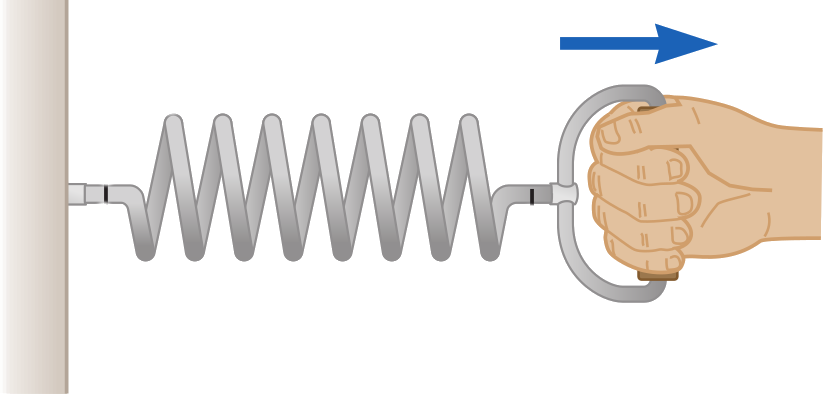
\includegraphics[scale=.18]{push_spring}};
					\draw[dashed] (-1.94,-.5)--(.76,-.5)--(.76,.6)--(-1.94,.6)--cycle;
					\end{tikzpicture}
					\caption{កម្លាំងទាញរ៉ឺស័រ}
				\end{subfigure}
				\begin{subfigure}[b]{0.3\textwidth}
					\centering
					\begin{tikzpicture}
					\node at (0,0) {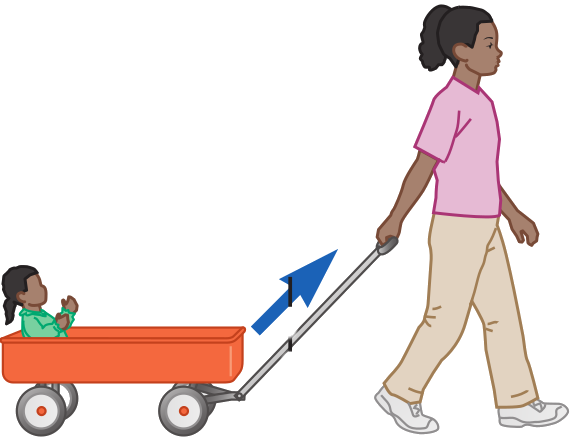
\includegraphics[scale=.25]{push_cart}};
					\draw[dashed] (-2.8,-2)--(1/20,-2)--(1/20,-.2)--(-2.8,-.2)--cycle;
					\end{tikzpicture}
					\caption{កម្លាំងទាញរទេះ}
				\end{subfigure}
				\begin{subfigure}[b]{0.3\textwidth}
					\centering
					\begin{tikzpicture}
					\node at (0,0) {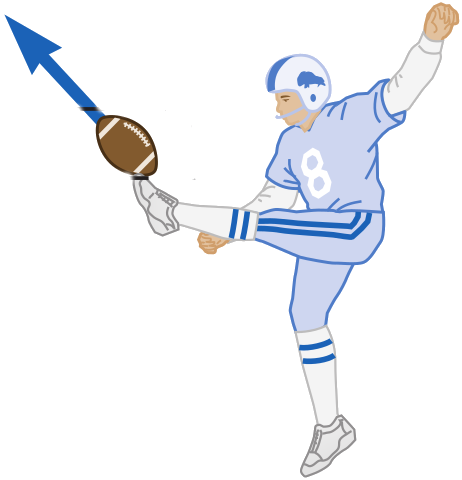
\includegraphics[scale=.25]{kick_ball}};
					\draw[dashed] (-1.5,.55)--(-.4,.55)--(-.4,1.15)--(-1.5,1.15)--cycle;
					\end{tikzpicture}
					\caption{កម្លាំងទាត់បាល់}
				\end{subfigure}
			\end{figure}
			\item \emph{\kml កម្លាំងពីចម្ងាយ ឬកម្លាំងដែន} ជាកម្លាំងដែលអង្គធាតុមួយបញ្ចេញលើអង្គធាតុមួយទៀត ដោយមិនចាំបាច់ប៉ះគ្នាផ្ទាល់។ ឧទាហរណ៍ កម្លាំងទំនាញផែនដី និងព្រះច័ន្ទ កម្លាំងអន្តរកម្មរវាងបន្ទុកអគ្គិសនីពីរដែលមានសញ្ញាដូចគ្នា ឬផ្ទុយគ្នា កម្លាំងឆក់ទាញដែកនៃមេដែក ជាដើម។ល។
			\begin{figure}[H]
				\centering
				\begin{subfigure}[b]{0.35\textwidth}
					\centering
					\begin{tikzpicture}
					\node at (0,0) {
\includegraphics[scale=.18]{earth}};
					\node at (-3,0) {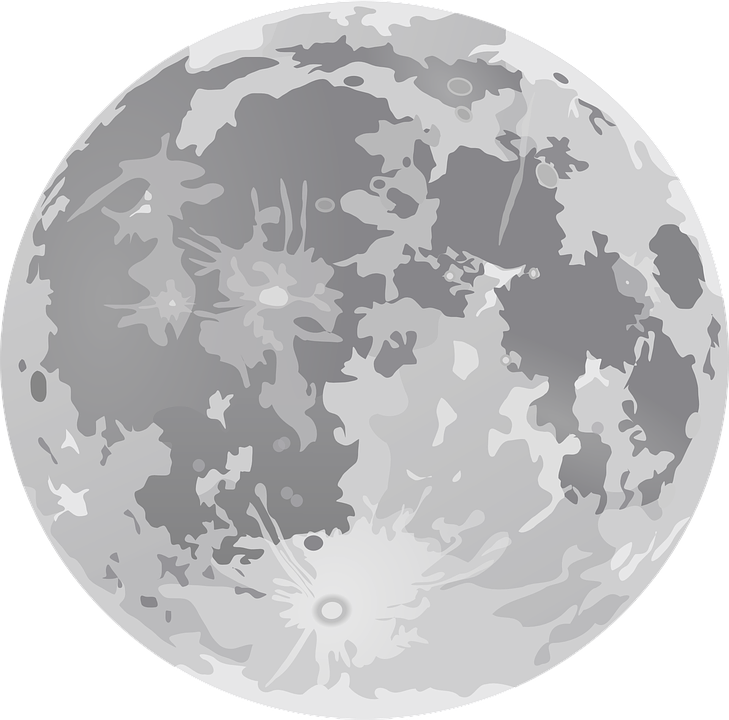
\includegraphics[scale=0.04]{moon}};
					\node at (0,-1.1) {$M_{\text{ផែនដី}}=5.9722\times10^{24}\si{\kilogram}$};
					\draw[dashed] (-3.7,-.6)--(-2.3,-.6)--(-2.3,.6)--(-3.7,.6)--cycle;
					\draw[->, line width=2pt, blue] (-2.5,0)--(-1.3,0);
					\node at (-1,1) {$M_{\text{ព្រះច័ន្ទ}}=7.342\times10^{22}\si{\kilogram}$};
					\end{tikzpicture}
					\caption{កម្លាំងទំនាញផែនដី និងព្រះច័ន្ទ}
				\end{subfigure}
				\begin{subfigure}[b]{0.32\textwidth}
					\centering
					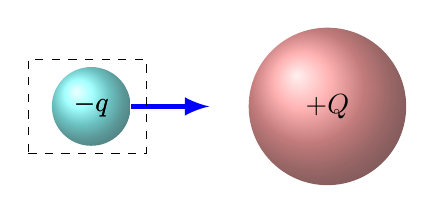
\begin{tikzpicture}
						\shade[ball color = cyan!60!white, opacity = 0.8] (-2,0) circle (.5cm);
						\node at (-2,0) {$-q$};
						\shade[ball color = red!50!white, opacity = 0.8] (1,0) circle (1cm);
						\node at (1,0) {$+Q$};
						\draw[->, line width=2pt, blue] (-1.5,0)--(-.5,0);
						\node at (-2,0) {$-q$};
						\draw[dashed] (-2.8,-.6)--(-1.3,-.6)--(-1.3,.6)--(-2.8,.6)--cycle;
					\end{tikzpicture}
					\caption{កម្លាំងអន្តរកម្មបន្ទុកអគ្គិសនីពីរ}
				\end{subfigure}
				\begin{subfigure}[b]{0.3\textwidth}
					\centering
					\begin{tikzpicture}
					\node at (0,0) {
\includegraphics[scale=.25]{magetic_bar}};
					\draw[dashed]
					 (-3.2,-.8)--(-.7,-.8)--(-.7,.7)--(-3.2,.7)--cycle;
					 \node at (-2.2,-.2) {\large\text{\kml ដែក}};
					\end{tikzpicture}
					\caption{កម្លាំងឆក់ទាញដែកនៃមេដែក}
				\end{subfigure}
			\end{figure}
		\end{enumerate}
	\end{enumerate}
\begin{exercise}
	\begin{enumerate}
		\item គេមានវ៉ិចទ័រកម្លាំងពីរដែលមានប្រវែង $4\si{\centi\metre}$ និង $9\si{\centi\metre}$។ តើកម្លាំងនីមួយៗ មានអាំងតង់ស៊ីតេប៉ុន្មាន?\\ បើគេយកមាត្រដ្ឋាន $2\si{\centi\metre}$ ត្រូវនឹង $30\si{\newton}$។
		\item ម៉ាស៊ីនស្ទូចមួយបានស្ទូចវត្ថុមួយមានទម្ងន់ $8000\si{\newton}$ ដោយល្បឿនថេរតាមរយខ្សែឈរ។\\ ចូរតាងកម្លាំងដែលម៉ាស៊ីនស្ទូចមានអំពើលើវត្ថុនោះដោយវ៉ិចទ័រតាមមាត្រដ្ឋាន $1\si{\centi\metre}$ ត្រូវនឹង $2000\si{\newton}$។
		\item កម្លាំងទាញលើក្បាលរទេះភ្លើងនៅផ្លូវដែកមួយស្មើនឹង $30000\si{\newton}$ និងកម្លាំងទប់លើរទេះភ្លើងស្មើនឹង $10000\si{\newton}$។\\ ចូរតាងកម្លាំងនោះដោយវ៉ិចទ័រតាមមាត្រដ្ឋាន $1\si{\centi\metre}$ ត្រូវនឹង $10000\si{\newton}$។
	\end{enumerate}
\end{exercise}
\subsection{ផលបូកកម្លាំង}
	\begin{enumerate}[k]
		\item \emph{\kml ករណីកម្លាំងទាំងពីរមានទិសដៅដូចគ្នា}
		បើយើងមានវ៉ិចទ័រកម្លាំងពីរគឺ $\overrightarrow{F}_{1}$ និង $\overrightarrow{F}_{2}$ មានទិស និងទិសដៅដូចគ្នា។ \\គេបានកម្លាំងផ្គួបនៃកម្លាំងទាំងពីរគឺ $ \overrightarrow{F}=\overrightarrow{F}_{1}+\overrightarrow{F}_{2}$
		លក្ខណៈសម្គាល់នៃកម្លាំងផ្គួប $\overrightarrow{F}$ គឺ៖
		\begin{flalign*}
			\text{ចំណុចចាប់}\quad :&\quad\text{នៅត្រង់}~O\\
			\text{ទិស}\quad :&\quad \text{ស្របគ្នា}\\
			\text{ទិសដៅ}\quad :&\quad \text{ដូចទិសដៅរបស់} \overrightarrow{F}_{1}~\text{និង}~ \overrightarrow{F}_{2}\\
			\text{អាំងតង់ស៊ីតេ}\quad :&\quad F=F_{1}+F_{2}
		\end{flalign*}
		\begin{figure}[H]
			\centering
			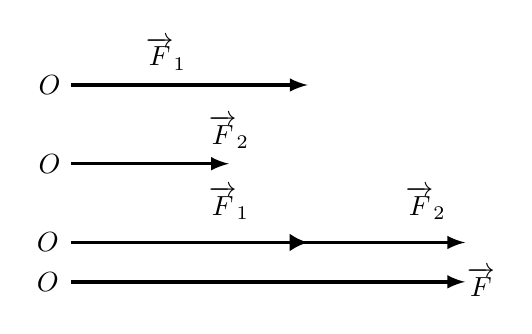
\begin{tikzpicture}
			\begin{scope}[very thick, every node/.style={sloped,allow upside down}]
			\coordinate[label=left:$O$] (O) at (0,2);
			\coordinate (A) at (3,2);
			\coordinate[label=left:$O$] (B) at (0,1);
			\coordinate (C) at (2,1);
			\coordinate (D) at (5,0);
			\draw [->] (O) -- (A);
			\draw [->] (B) -- (C);
			\draw [->] (0,0) -- (D);
			\draw [arrows = {-Latex[width=6.5pt, length=6.5pt]}] (2.8,0) -- (3,0);
			\draw (-.3,0) node {$O$};
			\draw (-.3,-.5) node {$O$};
			\draw (1.2,2.4) node {$\overrightarrow{F}_{1}$};
			\draw (2,1.4) node {$\overrightarrow{F}_{2}$};
			\draw (2,.5) node {$\overrightarrow{F}_{1}$};
			\draw (4.5,.5) node {$\overrightarrow{F}_{2}$};
			\draw [->] (0,-.5) -- (5,-.5);
			\draw (5.2,-.5) node {$\overrightarrow{F}$};
			\end{scope}
			\end{tikzpicture}
			\caption{ផលបូកវុិចទ័រក​​​ម្លាំង​​ពីរមានទិស និងទិសដៅដូចគ្នា}
		\end{figure}
		\item \emph{\kml ករណីកម្លាំងទាំងពីរមានទិសដៅផ្ទុយគ្នា}
		បើយើងមានវ៉ិចទ័រកម្លាំងពីរគឺ $\overrightarrow{F}_{1}$ និង $\overrightarrow{F}_{2}$ មានទិសដៅផ្ទុយគ្នា។ \\គេបានកម្លាំងផ្គួបនៃកម្លាំងទាំងពីរគឺ $ \overrightarrow{F}=\overrightarrow{F}_{1}+\overrightarrow{F}_{2}$
		លក្ខណៈសម្គាល់នៃកម្លាំងផ្គួប $\overrightarrow{F}$ គឺ៖
		\begin{flalign*}
			\text{ចំណុចចាប់}\quad :&\quad\text{នៅត្រង់}~O\\
			\text{ទិស}\quad :&\quad \text{ស្របគ្នា}\\
			\text{ទិសដៅ}\quad :&\quad \text{មានទិសដៅដូច}\\ 
			\quad:&\quad\overrightarrow{F}_{1}~\text{បើ}~F_{1}>F_{2}~\text{នោះ}~F=F_{1}-F_{2}\\
			\quad:&\quad\overrightarrow{F}_{2}~\text{បើ}~F_{1}<F_{2}~\text{នោះ}~F=F_{2}-F_{1}\\
			\text{អាំងតង់ស៊ីតេ}\quad :&\quad F=\abs{F_{1}-F_{2}}
		\end{flalign*}
		\begin{figure}[H]
			\centering
			\begin{tikzpicture}
				\coordinate[label=above:$O$] (O1) at (0,0);
				\coordinate[label=above:$O$] (O2) at (0,-1);
				\coordinate[label=above:$\overrightarrow{F}$] (F) at (1,-1);
				\coordinate[label=above:$\overrightarrow{F}_{1}$] (A) at (3,0);
				\coordinate[label=above:$\overrightarrow{F}_{2}$] (B) at (-2,0);
				\draw[->] (O1)--(A);
				\draw[->] (O1)--(B);
				\node at (O1) {$\bullet$};
				\node at (0,-1) {$\bullet$};
				\draw[->] (O2) -- (F);
				\draw[dashed] (O2) -- (-1,-1);
			\end{tikzpicture}
			\caption{ផលបូកវុិចទ័រក​​​ម្លាំង​​ពីរមានទិសដៅផ្ទុយគ្នា ករណី $F_{1}>F_{2}$}
		\end{figure}
		\begin{figure}[H]
			\centering
			\begin{tikzpicture}
			\coordinate[label=above:$O$] (O1) at (0,0);
			\coordinate[label=above:$O$] (O2) at (0,-1);
			\coordinate[label=above:$\overrightarrow{F}$] (F) at (-1,-1);
			\coordinate[label=above:$\overrightarrow{F}_{1}$] (A) at (2,0);
			\coordinate[label=above:$\overrightarrow{F}_{2}$] (B) at (-3,0);
			\draw[->] (O1)--(A);
			\draw[->] (O1)--(B);
			\node at (O1) {$\bullet$};
			\node at (0,-1) {$\bullet$};
			\draw[->] (O2) -- (F);
			\draw[dashed] (O2) -- (1,-1);
			\end{tikzpicture}
			\caption{ផលបូកវុិចទ័រក​​​ម្លាំង​​ពីរមានទិសដៅផ្ទុយគ្នា ករណី $F_{1}<F_{2}$}
		\end{figure}
		\item \emph{\kml ករណីកម្លាំងទាំងពីរមានទិសដៅកែងគ្នា} បើយើងមានវ៉ិចទ័រកម្លាំងពីរគឺ $\overrightarrow{F}_{1}$ និង $\overrightarrow{F}_{2}$ មានទិស និងទិសដៅកែងគ្នា។ \\គេបានកម្លាំងផ្គួបនៃកម្លាំងទាំងពីរគឺ $ \overrightarrow{F}=\overrightarrow{F}_{1}+\overrightarrow{F}_{2}$
		លក្ខណៈសម្គាល់នៃកម្លាំងផ្គួប $\overrightarrow{F}$ គឺ៖
		\begin{flalign*}
			\text{ចំណុចចាប់}\quad :&\quad\text{នៅត្រង់}~O\\
			\text{ទិស}\quad :&\quad \text{ស្ថិតលើអង្កត់ទ្រូងនៃចតុកោណកែង}\\
			\text{ទិសដៅ}\quad :&\quad \text{មានទិសដៅដូចរូបខាងក្រោម}\\
			\text{អាំងតង់ស៊ីតេ}\quad :&\quad F=\sqrt{F^2_{1}+F^2_{2}}
		\end{flalign*}
		\begin{figure}[H]
			\centering
			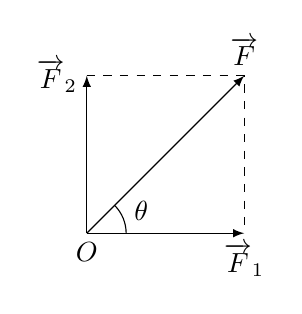
\begin{tikzpicture}
			\begin{scope}
			\coordinate[label=below:$O$] (O) at (0,0);
			\coordinate (F1) at (2,0);
			\coordinate (F2) at (0,2);
			\coordinate (F) at (2,2);
			\draw [->] (O) -- (F1);
			\draw [->] (O) -- (F2);
			\draw [->] (O) -- (F);
			\draw [dashed] (0,2) --(2,2) -- (2,0);
			\coordinate[label=below:$\overrightarrow{F}_{1}$] (F1) at (F1);
			\coordinate[label=left:$\overrightarrow{F}_{2}$] (F2) at (F2);
			\coordinate[label=above:$\overrightarrow{F}$] (F) at (F);
			\pic [draw, -, "$\theta$", angle eccentricity=1.5] {angle = F1--O--F};
			\end{scope}
			\end{tikzpicture}
			\caption{ផលបូកវុិចទ័រ​​កម្លាំង​​ពីរមានទិស និងទិសដៅកែងគ្នា}
		\end{figure}
		\item \emph{\kml ករណីកម្លាំងទាំងពីរមានទិសបង្កើតបានមុំ $\theta$} 
		បើយើងមានវ៉ិចទ័រកម្លាំងពីរគឺ $\overrightarrow{F}_{1}$ និង $\overrightarrow{F}_{2}$ មានទិស និងទិសដៅបង្កើតបានមុំ $\theta$ មួយ។ គេបានកម្លាំងផ្គួបនៃកម្លាំងទាំងពីរគឺ $ \overrightarrow{F}=\overrightarrow{F}_{1}+\overrightarrow{F}_{2}$
		លក្ខណៈសម្គាល់នៃកម្លាំងផ្គួប $\overrightarrow{F}$ គឺ៖
		\begin{flalign*}
		\text{ចំណុចចាប់}\quad :&\quad\text{នៅត្រង់}~O\\
		\text{ទិស}\quad :&\quad \text{ស្ថិតលើអង្កត់ទ្រូងនៃប្រលេឡូក្រាម}\\
		\text{ទិសដៅ}\quad :&\quad \text{មានទិសដៅដូចរូបខាងក្រោម}\\
		\text{អាំងតង់ស៊ីតេ}\quad :&\quad F=\sqrt{F^2_{1}+F^2_{2}-2F_{1}F_{2}\cos\left(\pi-\theta\right)}\\
		\text{ឬ}\quad :&\quad F =\sqrt{F^2_{1}+F^2_{2}+2F_{1}F_{2}\cos\theta}
		\end{flalign*}
		\begin{figure}[H]
			\centering
			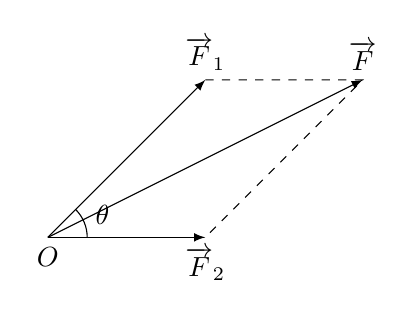
\begin{tikzpicture}
			\begin{scope}
			\coordinate[label=below:$O$] (O) at (0,0);
			\coordinate (01) at (2,0);
			\coordinate (F3) at (4,2);
			\coordinate (F1) at (2,2);
			\coordinate (F2) at (2,0);
			\coordinate (F) at (4,2);
			\draw [->] (O) -- (F1);
			\draw [->] (O) -- (F2);
			\draw [->] (O) -- (F);
			\draw [dashed] (2,2) --(4,2) -- (2,0);
			\coordinate[label=above:$\overrightarrow{F}_{1}$] (F1) at (F1);
			\coordinate[label=below:$\overrightarrow{F}_{2}$] (F2) at (F2);
			\coordinate[label=above:$\overrightarrow{F}$] (F) at (F);
			\pic [draw, -, "$\theta$", angle eccentricity=1.5] {angle = F2--O--F1};
			\end{scope}
			\end{tikzpicture}
			\caption{ផលបូកវុិចទ័រ​​កម្លាំង​​ពីរមានទិសបង្កើតបានមុំ $\theta$}
		\end{figure}
	\item \emph{\kml ករណីកម្លាំងច្រើនមានទិសជួបគ្នា}
		\begin{flalign*}
			\text{ផលបូកកម្លាំងរវាង $\overrightarrow{F}_{1}$ និង $\overrightarrow{F}_{2}$}\quad :&\quad \overrightarrow{F}=\overrightarrow{F}_{1}+\overrightarrow{F}_{2}\\
			\text{នោះ}\quad :&\quad \overrightarrow{R}=\overrightarrow{F}+\overrightarrow{F}_{3}\\
			\text{ឬ}\quad :&\quad \overrightarrow{R}=\overrightarrow{F}_{1}+\overrightarrow{F}_{2}+\overrightarrow{F}_{3}~\left(\overrightarrow{R}\text{ជាកម្លាំងផ្គួបនៃកម្លាំង} \overrightarrow{F}_{1},~\overrightarrow{F}_{2},~\overrightarrow{F}_{3}\right)
		\end{flalign*}
	\begin{figure}[H]
		\centering
		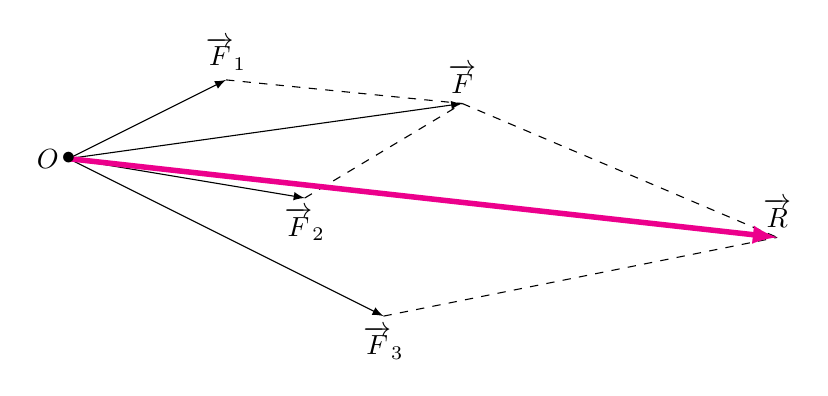
\begin{tikzpicture}
			\begin{scope}
				\coordinate[label=left:$O$] (O) at  (0,0);
				\coordinate[label=above:$\overrightarrow{F}_{1}$] (F1) at (2,1);
				\coordinate[label=below:$\overrightarrow{F}_{2}$] (F2) at (3,-.5);
				\coordinate[label=below:$\overrightarrow{F}_{3}$] (F3) at (4,-2);
				\coordinate[label=above:$\overrightarrow{F}$] (F) at (5,.7);
				\coordinate[label=above:$\overrightarrow{R}$] (R) at (9,-1);
				\draw[dashed] (F1) -- (F);
				\draw[dashed] (F2) -- (F);
				\draw[dashed] (F) -- (R);
				\draw[dashed] (F3) -- (R);
				\draw[->] (O) -- (F1);
				\draw[->] (O) -- (F2);
				\draw[->] (O) -- (F3);
				\draw[->] (O) -- (F);
				\draw[->, line width=2pt, magenta] (O) -- (R);
				\node at (O) {$\bullet$};
			\end{scope}
		\end{tikzpicture}
		\caption{ករណីមានវ៉ិចទ័រកម្លាំងច្រើនមានទិសជួបគ្នា}
	\end{figure}
	\end{enumerate}
	\begin{remark}
		ដើម្បីសង់វុិចទ័រកម្លាំងផ្គួប $\overrightarrow{F}$ ដែល $\overrightarrow{F}=\overrightarrow{F}_{1}+\overrightarrow{F}_{2}$ យើងត្រូវអនុវត្តតាមវិធានអង្តត់ទ្រូងប្រលេឡូក្រាម។
	\end{remark}
\begin{exercise}
	\begin{enumerate}[m]
		\item កម្លាំងខាងក្រោមនេះ ធ្វើអំពើលើចំណុចមួយនៃអង្គធាតុមួយ៖
		\begin{itemize}
			\item កម្លាំង $17\si{\newton}$ មានទិសឈរ និងមានទិសដៅពីក្រោមឡើងលើ
			\item កម្លាំង $11\si{\newton}$ មានទិសឈរ និងមានទិសដៅពីលើចុះក្រោម
			\item កម្លាំង $18\si{\newton}$ មានទិសដេក និងមានទិសដៅពីឆ្វេងទៅស្តាំ
			\item កម្លាំង $10\si{\newton}$ មានទិសដេក និងមានទិសដៅពីស្តាំទៅឆ្វេង។
		\end{itemize}
		រកកម្លាំងផ្គួបនៃកម្លាំងទាំងនោះ។
		\item កំណត់កម្លាំងផ្គួបនៃកម្លាំងពីរដែលមានអាំងតង់ស៊ីតេស្មើគ្នាហើយមុំបង្កើតដោយកម្លាំងទាំងពីរស្មើនឹង $60^{\circ}$។
		\item កំណត់កម្លាំងផ្គួបនៃកម្លាំងពីរដែលមានអាំងតង់ស៊ីតេស្មើគ្នា។\\ គេដឹងថាមុំដែលបង្កើតដោយកម្លាំងទាំងពីរស្មើនឹង $120^{\circ}$។
		\item កំណត់កម្លាំងផ្គួបនៃកម្លាំងជួបបីដែលមានអាំងតង់ស៊ីតេស្មើគ្នាឋិតក្នុងប្លង់តែមួយ ហើយបង្កើតបានមុំ $120^{\circ}$ ពីកម្លាំងមួយទៅកម្លាំងមួយទៀត(ដូចរូប)។
		\begin{figure}[H]
			\centering
			\begin{tikzpicture}[>=Stealth]
			\coordinate (O) at (0,0);
			\coordinate[label=below:$F_{1}$] (F1) at (0,-3);
			\coordinate[label=above:$F_{2}$] (F2) at (3, 1);
			\coordinate[label=above:$F_{3}$] (F3) at (-3, 1);
			\draw[->, magenta] (O)--(F1);
			\draw[->, magenta] (O)--(F2);
			\draw[->, magenta] (O)--(F3);
			\pic [draw, -, "$120^{\circ}$", angle eccentricity=2.5, angle radius=.3cm] {angle = F1--O--F2};
			\pic [draw, -, "$120^{\circ}$", angle eccentricity=2.5, angle radius=.3cm] {angle = F2--O--F3};
			\pic [draw, -, "$120^{\circ}$", angle eccentricity=2.5, angle radius=.3cm] {angle = F3--O--F1};
			\end{tikzpicture}
		\end{figure}
	\item ចូរគូសរូបដើម្បីរកកម្លាំងផ្គួបនៃកម្លាំងទាំងពីរគឺ $294\si{\newton}$ និង $392\si{\newton}$ ដែលបញ្ចេញលើអង្គធាតុមួយព្រមគ្នា និងមានទិសបង្កើតបានមុំ៖ $30^\circ,~60^\circ,~90^\circ$ និង $120^\circ$។ គណនាអាំងតង់ស៊ីតេនៃកម្លាំងផ្គួប។
	\end{enumerate}
\end{exercise}
\subsection{បំបែកកម្លាំង} កម្លាំងទោលមួយអាចបំបែកជាកម្លាំងផ្គុំពីរឬច្រើនដែលផ្តល់ផលដូចគ្នានឹងកម្លាំងទោលដោយប្រើវិធានប្រលេឡូក្រាម។
\begin{enumerate}
	\item \emph{\kml បំបែកកម្លាំងមួយជាកម្លាំងពីរកែងគ្នា}
	\begin{flalign*}
		\text{ជាវ៉ិចទ័រ}\quad :&\quad \overrightarrow{F}=\overrightarrow{F}_{x}+\overrightarrow{F}_{y}\\
		\text{ជាតម្លៃ}\quad :&\quad F=\sqrt{F^2_{x}+F^2_{y}}\quad
		\text{ដែល}\quad F_{x}=F\cos\theta~\text{និង}~F_{y}=F\sin\theta
	\end{flalign*}
	\begin{figure}[H]
		\centering
		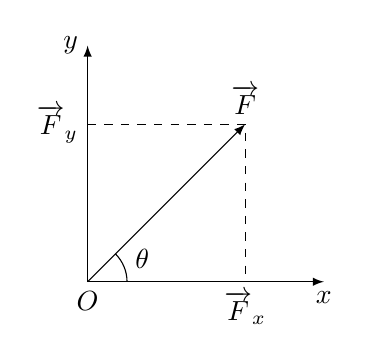
\begin{tikzpicture}
		\begin{scope}
		\coordinate (O) at (0,0);
		\coordinate (x) at (3,0);
		\coordinate (y) at (0,3);
		\coordinate (F) at (2,2);
		\draw [->] (O) -- (x);
		\draw [->] (O) -- (y);
		\draw [->] (O) -- (F);
		\draw [dashed] (0,2) --(2,2) -- (2,0);
		\coordinate[label=below:$x$] (x) at (x);
		\coordinate[label=left:$y$] (y) at (y);
		\coordinate[label=above:$\overrightarrow{F}$] (F) at (F);
		\coordinate[label=below:$\overrightarrow{F}_{x}$] (Fx) at (2,0);
		\coordinate[label=left:$\overrightarrow{F}_{y}$] (Fy) at (0,2);
		\coordinate[label=below:$O$] (0,0) at (0,0);
		\pic [draw, -, "$\theta$", angle eccentricity=1.5] {angle = x--O--F};
		\end{scope}
		\end{tikzpicture}
		\caption{បំបែកកម្លាំងមួយជាកម្លាំងពីរកែងគ្នា}
	\end{figure}
	\item \emph{\kml បំបែកកម្លាំងមួយជាកម្លាំងពីរស្របគ្នា}
	\begin{figure}[H]
		\centering
		\begin{tikzpicture}
			\begin{scope}
				\draw[->] (.5,0)--(.5,-2);
				\draw[->] (7.5,0)--(7.5,-2);
				\fill[top color=gray, bottom color=gray!40!white] (0,0) rectangle (8,.3);
				\shade[bottom color=fancyorange1, top color=fancyorange2] (.5,0)--(-.5,-1)--(1.5,-1)--cycle;
				\shade[bottom color=fancyorange1, top color=fancyorange2] (7.5,0)--(8.5,-1)--(6.5,-1)--cycle;
				\shade[bottom color=fancyorange1, top color=fancyorange2] (5,.3)--(6,.3)--(6,1.5)--(5,1.5)--cycle;
				\node at (5.5,.8) {$\bullet$};
				\draw[->,line width=2pt] (5.5,.8)--(5.5,-2);
				\draw[<->] (.5,1)--(5,1);
				\draw[<->] (6,1)--(7.5,1);
				\node at (2.5,1.2) {$d_{1}$};
				\node at (6.7,1.2) {$d_{2}$};
				\node at (1,-1.8) {$\overrightarrow{F}_{1}$};
				\node at (6,-1.8) {$\overrightarrow{F}$};
				\node at (8,-1.8) {$\overrightarrow{F}_{2}$};
			\end{scope}
		\end{tikzpicture}
		\caption{បំបែកកម្លាំងមួយជាកម្លាំងពីរស្របគ្នា}
	\end{figure}
	\begin{flalign*}
		\text{ជាវ៉ិចទ័រ}\quad :&\quad \overrightarrow{F}=\overrightarrow{F}_{1}+\overrightarrow{F}_{2}\\
		\text{ជាម៉ូឌុល}\quad :&\quad F=F_{1} + F_{2}\\
		\text{ម្យ៉ាងទៀត}\quad :&\quad F_{1}\times d_{1}=F_{2}\times d_{2}~\text{ឬ}~\frac{F_{1}}{F_{2}}=\frac{d_{2}}{d_{1}}
	\end{flalign*}
\end{enumerate}
\begin{exercise}
	\begin{enumerate}
		\item កម្លាំង $10\si{\newton}$ មានទិសបង្កើតបាន $37^\circ$ ធៀបនឹងទិសដេក។ រកកម្លាំងផ្គុំឈរ និងកម្លាំងផ្គុំដេករបស់វា។
		\item គេដំដែកគោលមួយលើជញ្ជាំងតាមមុំ $45^\circ$ នឹងប្លង់ជញ្ជាំងឈរដោយកម្លាំង $30\si{\newton}$។\\
		រកអាំងតង់ស៊ីតេកម្លាំងផ្គុំតាមទិសដេក និងទិសឈរ។
	\end{enumerate}
\end{exercise}
\section{ច្បាប់ចលនារបស់ញូតុន}
\subsection{ច្បាប់ទី១ ញូតុន ឬ ច្បាប់និចលភាព}
\begin{itemize}
	\item \emph{\kml ច្បាប់ទី១ ញូតុនពោលថាៈ} កាលណាអង្គធាតុមួយមិនរងអំពើនៃកម្លាំងផ្សេងៗទេ ឬវារងកម្លាំងផ្គួបស្មើនឹងសូន្យ នោះបើវានៅនឹងថ្កល់ស្រាប់វានឹងនៅតែនឹងថ្កល់ដដែល តែបើវាមានចលនាស្រាប់ ចលនានោះជាចលនាត្រង់ស្មើ។
	\item \emph{\kml និចលភាព} ជាលក្ខណៈនៃគ្រប់អង្គធាតុដែលចង់រក្សាភាពមានចលនា ឬភាពនៅនឹងថ្កល់របស់វា។ គេអាចនិយាយម្យ៉ាងទៀតថា លក្ខណៈរក្សាល្បឿននៃអង្គធាតុហៅថា និចលភាព ហើយចលនាត្រង់ស្មើហៅថា ចលនាដោយនិចលភាព។
	\item \emph{\kml ច្បាប់ទី១ ញូតុន គេអាចសរសេរ} $\Sigma \overrightarrow{F}=\overrightarrow{0}$
\end{itemize}
\begin{remark}
	ក្នុងភាពលំនឹងមានន័យថា វត្ថុអាចនៅនឹងថ្កល់ ឬក៏កំពុងផ្លាស់ទីលើគន្លងត្រង់ដោយវ៉ិចទ័រល្បឿនថេរ(ចលនាត្រង់ស្មើ)។ លក្ខណៈបែបនេះ ហៅថានិចលភាព។
\end{remark}
\subsection{ច្បាប់ទី២ ញូតុន ឬ ច្បាប់គ្រឹះឌីណាមិច}
\begin{itemize}
	\item \emph{\kml ច្បាប់ទី២ ញូតុនពោលថាៈ} នៅពេលកម្លាំងសរុបដែលមានអំពើលើវត្ថុមួយមិនស្មើសូន្យ វត្ថុនឹងស្ទុះតាមទិសដៅកម្លំាងដែលបានប្រព្រឹត្តលើវា ហើយសំទុះសមាមាត្រដោយផ្ទាល់នឹងកម្លាំងសរុប ដែលមានអំពើលើវាហើយ ច្រាសសមាមាត្រនឹងម៉ាសរបស់វា។
	\begin{flalign*}
		\text{សំទុះនៃចលនារបស់អង្គធាតុសមាមាត្រនឹងកម្លាំងផ្គួប}\quad :&\quad \overrightarrow{a}\propto\Sigma \overrightarrow{F}\\
		\text{សំទុះនៃចលនារបស់អង្គធាតុច្រាសសមាមាត្រនឹងកម្លាំងផ្គួប}\quad :&\quad \overrightarrow{a}\propto\frac{1}{m}\\
		\text{គេបាន}\quad :&\quad \overrightarrow{a}=\frac{\Sigma \overrightarrow{F}}{m}~\text{ឬ}~\Sigma\overrightarrow{F}=m\overrightarrow{a}\\
		\text{ជាម៉ូឌុល}\quad :&\quad \Sigma F=ma~\left(\overrightarrow{F}~\text{និង}~\overrightarrow{a}~\text{មានទិសដៅដូចគ្នា}\right)
	\end{flalign*}
	\begin{remark}
		\begin{itemize}
			\item បើកម្លាំង $\overrightarrow{F}$ ថេរ នាំឲ្យសំទុះថេរ៖ អង្គធាតុមានចលនាត្រង់ប្រែប្រួលស្មើ។
			\item បើកម្លាំង $\overrightarrow{F}$ ថេរ និងមានទិសដៅដូចល្បឿន៖ អង្គធាតុមានចលនាត្រង់ស្ទុះស្មើ។
			\item បើកម្លាំង $\overrightarrow{F}$ ថេរ និងទិសដៅផ្ទុយពីល្បឿន៖ អង្គធាតុមានចលនាត្រង់យឺតស្មើ
			\item បើកម្លាំង $\overrightarrow{F}=\overrightarrow{0}$ និងមាន $\overrightarrow{a}=\overrightarrow{0}$៖ អង្គធាតុមានចលនាត្រង់ស្មើ។ 
		\end{itemize}
	\end{remark}
\end{itemize}
\begin{exercise}
	\begin{enumerate}
		\item ក្មេងប្រុសម្នាក់រុញប្រអប់មួយដែលមានម៉ាស $10\si{\kilogram}$ ដោយកម្លាំង $20\si{\newton}$។ តើសំទុះនៃប្រអប់ស្មើនឹងប៉ុន្មាន? កកិតអាចចោលបាន។
		\item រថយន្តមួយមានម៉ាស $1.0\times10^{3}\si{\kilogram}$ មានចលនាស្ទុះស្មើដោយចាប់ផ្តើមពីល្បឿនសូន្យទៅល្បឿន $20\si{\metre/\second}$ ក្នុងរយៈពេល $10\si{\second}$។ គណនាកម្លាំងម៉ាស៊ីនដែលរថយន្តបញ្ចេញដើម្បីឲ្យវាទៅមុខ។ កម្លាំងកកិតអាចចោលបាន។ 
		\item គណនាកម្លាំងចំបាច់ ដើម្បីឲ្យវត្ថុមួយមានម៉ាស $48\si{\kilogram}$ មានសំទុះ $6\si{\metre/\second^{2}}$។
		\item កម្លាំង $200\si{\gram\cdot\centi\metre/\second^{2}}$ បញ្ជូនសំទុះ $500\si{\centi\metre/\second^{2}}$ ឲ្យវត្ថុមួយ។ គណនាម៉ាសនៃវត្ថុនោះ។
		\item កម្លាំង $0.20\si{\newton}$ មានអំពើលើវត្ថុមួយដែលមានម៉ាស $100g$។ គណនាសំទុះនៃវត្ថុនោះ។
		\item កម្លាំង $\SI{e-2}{\newton}$ មានអំពើលើវត្ថុមួយដែលមានម៉ាស $1\si{\gram}$។\\ តើមួយវិនាទីក្រោយមក វត្ថុនោះផ្លាស់ទីបានចម្ងាយប៉ុន្មានម៉ែត្រ? តើ $5\si{\second}$ ក្រោមមកវាមានល្បឿនប៉ុន្មាន?
		\item កម្លាំងថេរមួយមានអំពើលើវត្ថុមួយមានម៉ាស $300\si{\gram}$ ធ្វើឲ្យវត្ថុនោះចេញពីស្ថានភាពនៅស្ងៀមហើយផ្លាស់ទីបានចម្ងាយ $25\si{\meter}$ ក្នុងរយៈពេល $5\si{\second}$។ គណនាកម្លាំងនោះ។
		\item កូនបាល់មួយមានម៉ាស $100\si{\gram}$ កំពុងឋិតនៅស្ងៀម ហើយរងកម្លាំងមួយថេរស្មើនឹង $200\si{\gram\cdot\centi\metre/\second^{2}}$ ក្នុងរយៈពេល $10\si{\second}$។ គណនាល្បឿនរបស់បាល់ និងចម្ងាយដែលវាផ្លាស់ទីបានក្នុងរយៈពេល $10\si{\second}$។
	\end{enumerate}
\end{exercise}
\subsection{ច្បាប់ទី៣ ញូតុន ឬ ច្បាប់អំពើ និងប្រតិកម្ម}
\begin{itemize}
	\item \emph{\kml ច្បាប់ទី៣ ញូតុនពោលថាៈ} នៅពេល វត្ថុទី១បញ្ចេញកម្លាំងមួយទៅលើវត្ថុទី២ នោះវត្ថុទី២ ក៏បញ្ចេញកម្លាំងមួយមកលើវត្ថុទី១ វិញដែរ ដែលមានតម្លៃស្មើគ្នា ប៉ុន្តែមានទិសដៅផ្ទុយគ្នា។
	\begin{flalign*}
		\text{កម្លាំងអំពើ~$\overrightarrow{F}_{12}$}\quad :&\quad \text{ជាកម្លាំងដែលវត្ថុទី១ បញ្ចេញលើវត្ថុទី២}\\
		\text{កម្លាំងប្រតិកម្ម~$\overrightarrow{F}_{21}$}\quad :&\quad \text{ជាកម្លាំងដែលវត្ថុទី២ បញ្ចេញលើវត្ថុទី១}
	\end{flalign*}
	\item \emph{\kml ច្បាប់ទី៣ ញូតុនបង្ហាញលក្ខណៈសម្គាល់បួនយ៉ាងនៃកម្លាំង មានដូចជា៖}
	\begin{itemize}
		\item [$-$] កម្លាំងកើតឡើងជាគូ។ គូកម្លាំងនេះហៅថា អំពើ និងប្រតិកម្ម។
		\item [$-$] អំពើ និងប្រតិកម្មមាន អាំងតង់ស៊ីតេស្មើគ្នា។
		\item [$-$] អំពើ និងប្រតិកម្មមានទិសដៅផ្ទុយគ្នា។
		\item [$-$] អំពើ និងប្រតិកម្មមានចំណុចចាប់លើអង្គធាតុពីរផ្សេងគ្នា ដូចនេះ វាមិនមែនជាកម្លាំងលំនឹងទេ។
	\end{itemize}
	\item \emph{\kml ច្បាប់ទី៣ ញូតុន គេអាចសរសេរ} $\overrightarrow{F}_{12}=-\overrightarrow{F}_{21}$ ជាតម្លៃ $F_{12}=F_{21}$
	\begin{figure}[H]
		\centering
		\begin{tikzpicture}
			\node at (0,0) {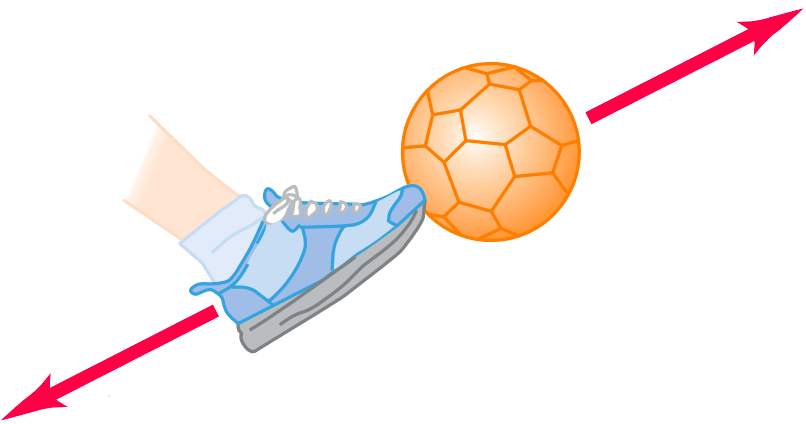
\includegraphics[scale=.2]{third_law_newton}};
			\node at (-2,-1.7) {$\vec{F}_{\text{បាល់មានអំពើលើជើង}}$};
			\node at (4,.8) {$\vec{F}_{\text{ជើងមានអំពើលើបាល់}}$};
		\end{tikzpicture}
		\caption{កម្លាំងជើងនិងបាល់បញ្ចេញអន្តរកម្មលើគ្នាទៅវិញទៅមក ដែលមានទំហំស្មើគ្នា ក្នុងទិសដៅផ្ទុយ}
	\end{figure}
\end{itemize}
\section{ម៉ាស និងទម្ងន់}
\subsection{ម៉ាស{\en(Mass)}}
\begin{definition}
	ម៉ាសនៃអង្គធាតុមួយ ជាទំហំអាស្រ័យតែនឹងអង្គធាតុនោះផ្ទាល់ ហើយមានឥទ្ធិពលដល់ទម្ងន់របស់អង្គធាតុនោះ។ អង្គធាតុមួយមានម៉ាសកំណត់។ បើម៉ាសនៃអង្គធាតុកាន់តែធំ នោះនិចលភាពនៃអង្គធាតុនោះ ក៏កាន់តែធំដែរ។ ដូចនេះ ម៉ាសជាទំហំកំណត់និចលភាពនៃវត្ថុ។
\end{definition}
\subsection{ទម្ងន់ ឬកម្លាំងទំនាញដែនដី{\en(Weight or Gravitational Force)}}
\begin{definition}
	 ទម្ងន់ ឬកម្លាំងទំនាញផែនដី ជាកម្លាំងដែលផែនដីទាញវត្ថុ ហើយមានទិសដៅតម្រង់មករកផ្ចិតនៃផែនដី។\\
	 ដើម្បីគណនាទម្ងន់នៃអង្គធាតុមួយ យើងប្រើរូបមន្ត $\vec{w}=m\vec{g}$ ជាម៉ូឌុល $w=mg$ ដែល $g$ ជាសំទុះទំនាញផែនដី។
\end{definition}
\begin{remark}
	\begin{enumerate}[k,2]
		\item ម៉ាសបង្ហាញពីបរិមាណរូបធាតុដែលបង្កើតវត្ថុ។
		\item ទម្ងន់បង្ហាញពីទំហំរបស់ទំនាញ។
	\end{enumerate}
\end{remark}
\subsection{ភាពខុសគ្នារវាង ម៉ាស និងទម្ងន់}
\begin{center}
	\begin{tabular}{|l|l|}
		\hline
		\multicolumn{1}{|c|}{{\cellcolor[HTML]{96FFFB}\ak ម៉ាស}} & \multicolumn{1}{|c|}{{\cellcolor[HTML]{96FFFB}\ak ទម្ងន់}}\\
		\hline
		- ជាបរិមាណរូបធាតុមាននៅក្នុងអង្គធាតុ & 	
		- ជាកម្លាំងទំនាញផែនដី \\ 
		- មានតែតម្លៃ គ្មានទិសដៅ & 
		- មានតម្លៃ និងទិសដៅ\\ 
		- មានខ្នាត់គិតជាគីឡូក្រាម $\left(\si{\kilogram}\right)$ &
		- មានខ្នាត់គិតជាញូតុន $\left(\si{\newton}\right)$\\
		- មានតម្លៃថេរគ្រប់ទីកន្លែង &
		- ប្រែប្រួលតាមទីកន្លែង\\
		- វាស់ដោយជញ្ជីង & 
		- វាស់ដោយឌីណាម៉ូម៉ែត្រ\\
		\hline
	\end{tabular}
\end{center}
\begin{figure}[H]
	\centering
	\begin{subfigure}[b]{0.45\textwidth}
		\centering
		\begin{tikzpicture}
			\node at (0,0) {
\includegraphics[scale=.25]{mass_on_earth}};
			\draw[->, line width=2pt, magenta] (-1.3,-2.4)--(-1.3,-4.5);
			\draw[->, line width=2pt, blue] (-1,-2.4)--(-1,-3.5);
			\node at (1,-2) {\text{ម៉ាស}~$m=1.00\si{\kilogram}$};
			\node at (1.5,-3) {\text{សំទុះទំនាញដី}~$g=9.80\si{\meter/\second^{2}}$};
			\node at (-3,-4) {\text{ទម្ងន់}~$w=9.80\si{\newton}$};
		\end{tikzpicture}
		\caption{ម៉ាស និងទម្ងន់របស់វត្ថុស្ថិតនៅលើផែនដី}
	\end{subfigure}
	\begin{subfigure}[b]{0.45\textwidth}
		\centering
		\begin{tikzpicture}
		\node at (0,0) {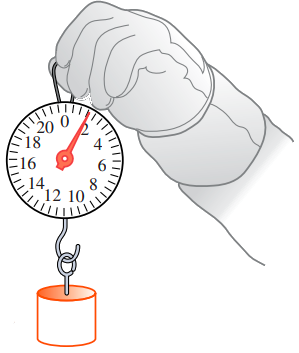
\includegraphics[scale=.35]{mass_on_the_moon}};
		\draw[->, line width=2pt, blue] (-.9,-2.1)--(-.9,-2.8);
		\draw[->, line width=2pt, magenta] (-1.2,-2.1)--(-1.2,-3);
		\node at (1,-1.8) {\text{ម៉ាស}~$m=1.00\si{\kilogram}$};
		\node at (1.8,-2.8) {\text{សំទុះទំនាញ}~$g=1.62\si{\meter/\second^{2}}$};
		\node at (-3,-3) {\text{ទម្ងន់}~$w=1.62\si{\newton}$};
		\end{tikzpicture}
		\caption{ម៉ាស និងទម្ងន់របស់វត្ថុស្ថិតនៅលើឋានព្រះច័ន្ទ}
	\end{subfigure}
\end{figure}
\begin{remark}
	ម៉ាសរបស់វត្ថុមួយមានតម្លៃថេរជានិច្ច ប៉ុន្តែទម្ងន់របស់វាប្រែប្រួលតាមទីកន្លែងដែលវាស្ថិតនៅ។
\end{remark}
\begin{exercise}
	\begin{enumerate}
		\item អង្គធាតុមួយមានទម្ងន់ $100\si{\newton}$ នៅលើផែនដី។ បើគេយកអង្គធាតុនោះទៅកាន់ភពមួយដែលមានសំទុះទំនាញស្មើនឹង $2\si{\metre/s^2}$។ តើអង្គធាតុនោះមានទម្ងន់ប៉ុន្មាននៅលើភពនោះ?
		\item នៅចុងខ្សែមួយបានចងភ្ជាប់នឹងកូនជញ្ជីង $50\si{\kilogram}$។ គេទាញកូនជញ្ជីងចេញពីទីតាំងលំនឹងបានមុំ $30^\circ$។\\ រកកម្លាំងដែលទាញកូនជញ្ជីងពីទីតាំងលំនឹង និងតំណឹងនៃខ្សែ។
		\begin{figure}[H]
			\centering
			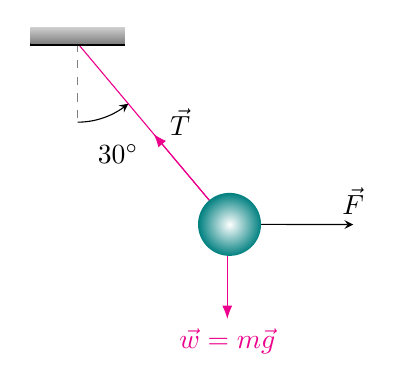
\begin{tikzpicture}[>=stealth]
			\begin{scope}
				\coordinate (centre) at (0,0);
				\coordinate (force) at (3.5,-2.3);
				\draw[dashed,gray] (centre) -- ++ (0,-1) node (mary) [black,below]{$ $};
				\draw[magenta] (centre) -- ++(310:3) coordinate (block);
				\draw[->] (block)--(force) node[above] (force) {$\vec{F}$};
				\draw[<-, magenta, >=Latex] (310:1.5) -- (block);
				\draw[->, magenta, >=Latex] (1.9,-2.5) -- (1.9,-3.5) node[below] (1.9,-3.5) {$\vec{w}=m\vec{g}$};
				\node[circle,outer color=teal,inner color=white,minimum width=.8cm] (radial) at (block) {};
				\pic [draw, ->, "$30^\circ$", angle eccentricity=1.5, angle radius=1cm] {angle = mary--centre--block};
				\draw [line width=2pt] (-.6,0) -- (.6,0);
				\fill[bottom color=gray, top color=gray!40!white] ($ (centre) + (-.6,0) $) rectangle ($ (centre) + (.6,0.2) $);
				\coordinate (m) at (block);
				\node at (1.3,-1) {$\vec{T}$};
			\end{scope}
			\end{tikzpicture}
		\end{figure}
	\item តំណក់ទឹកភ្លៀងជាមធ្យមមានម៉ាស $0.05\si{\gram}$។ ដោយសារខ្យល់បក់តាមទិសដេក ទើបតំណក់ទឹកភ្លៀងធ្លាក់ចុះមកដីតាមទិសដែលធ្វើបានមុំ $60^\circ$ ជាមួយប្លង់ដេក។ រកកម្លាំងខ្យល់បក់លើតំណក់ទឹកភ្លៀង។
	\item គេព្យួរវត្ថុមួយដែលមានម៉ាស $60\si{\kilogram}$ ទៅនឹងចុងខ្សែពីរដែលទិសវាបង្កើតបានមុំ $ABC$ ស្មើនឹង $120^\circ$(ដូចរូប)។\\ រកតំណឹងនៃខ្សែទាំងពីរគឺខ្សែ $AB$ និងខ្សែ $BC$។
	\begin{figure}[H]
		\centering
		\begin{tikzpicture}[>=stealth, decoration=rope]
		\begin{scope}
		\coordinate[label=below left:{$A$}] (A) at (0,0);
		\coordinate[label=below left:{$B$}] (B) at (2,-2);
		\coordinate[label=below left:{$C$}] (C) at (4,-2);
		\coordinate (T1) at (1.8,-1);
		\coordinate (block) at (2,-2.5);
		\draw[gray,thin,decorate,rope width=3pt] (A) -- (B);
		\draw[gray,thin,decorate,rope width=3pt] (B) -- (C);
		\draw[gray,thin,decorate,rope width=3pt] (B) -- (block);
		\node at (A) {$\bullet$};
		\node at (B) {$\bullet$};
		\node at (C) {$\bullet$};
		\node[circle,outer color=gray,inner color=white,minimum width=.1cm] (radial) at (B) {};
%		\coordinate[label=above:{$\vec{T}_{BC}$}] (T2) at (3,-2);
		\fill[bottom color=gray, top color=gray!40!white] ($ (A) + (-.6,0) $) rectangle ($ (A) + (.6,0.3) $);
		\fill[left color=gray, right color=gray!40!white] ($ (C) + (0,-.5) $) rectangle ($ (C) + (.3,.5) $);
%		\node at (T1) {$\vec{T}_{AB}$};
		\node at (block) {$\bullet$};
		\shade[top color=teal,bottom color=teal,middle color=white, fill opacity=1.0, rounded corners] (1.5,-3.5) rectangle (2.5,-2.5);
		\pic [draw, ->, "$120^\circ$", angle eccentricity=1.5, angle radius=.5cm] {angle = C--B--A};
		\node at (2,-3) {$60\si{\kilogram}$};
		\end{scope}
		\end{tikzpicture}
	\end{figure}
	\end{enumerate}
\end{exercise}
\section{កម្លាំងកែង និងកម្លាំងកកិត}
\subsection{កម្លាំងកែង ឬកម្លាំងប្រតិកម្មកែង{\en (Normal Force)}}
\quad មុនយើងនិយាយពីកម្លាំងកកិត យើងនឹងរៀនអំពីកម្លាំងថ្មីមួយទៀត ហៅថាកម្លាំងកែង។ កម្លាំងកែង មានអំពើលើវត្ថុដែលប៉ះនឹងផ្ទៃ។ វាមានអំពើកែងជានិច្ចនឹងផ្ទៃប៉ះ។ គេតាងវ៉ិចទ័រកម្លាំងកែងដោយ $\vec{F}_{N}$
\begin{figure}[H]
	\centering
	\begin{subfigure}[b]{0.4\textwidth}
		\centering
		\begin{tikzpicture}
		\node at (0,0) {
\includegraphics[scale=.2]{normal_force1}};
		\node at (.4,1) {$\vec{F}_{N}$};
		\end{tikzpicture}
		\caption{កម្លាំងកែងលើប្លង់ដេក}
	\end{subfigure}
	\begin{subfigure}[b]{0.4\textwidth}
		\centering
		\begin{tikzpicture}
		\node at (0,0) {
\includegraphics[scale=.2]{normal_force2}};
		\node at (1.4,1) {$\vec{F}_{N}$};
		\end{tikzpicture}
		\caption{កម្លាំងកែងលើប្លង់ទេរ}
	\end{subfigure}
\end{figure}
\begin{flalign*}
	\text{រូបមន្តដើម្បីគណនាកម្លាំងកែងគឺ}\quad :&\quad \vec{F}_{N}=-\vec{w}=-m\vec{g}~\text{(ប្លង់ដេក)}\\
	\text{ជាម៉ូឌុល}\quad :&\quad F_{N}=w=mg\\
\end{flalign*}
\subsection{កម្លាំងកកិត​{\en (Friction Forces)}}
\quad ឥឡូវ យើងនឹងនិយាយអំពីកកិត។ ឧបមាថាយើងរុញសៀវភៅមួយក្បាលក្រោមល្បឿនថេរ ដោយកម្លាំង $\vec{F}$ លើផ្ទៃតុមួយ នោះយើងនឹងសង្កេតឃើញថាកកិតរវាងផ្ទៃតុ នឹងសៀវភៅកើតមានឡើង។ កម្លាំងដែលកើតឡើងដោយសារកកិតរវាងវត្ថុពីរនោះហៅថាកម្លាំងកកិតដែលតាងដោយ $\vec{f}$ ហើយមានទិសដៅផ្ទុយនឹងកម្លាំងដែលកំពុងរុញសៀវភៅនោះគឺ $\vec{F}$។
\begin{figure}[H]
	\centering
	\begin{tikzpicture}
		\node at (0,0) {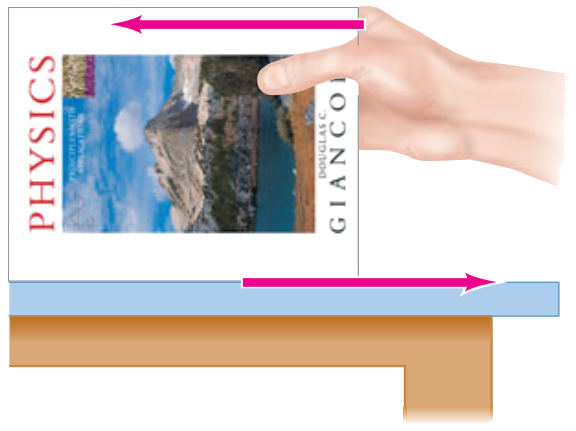
\includegraphics[scale=.3]{push_book}};
		\node at (-1.5,2.5) {$\vec{F}$};
		\node at (2,-.2) {$\vec{f}$};
	\end{tikzpicture}
	\caption{កម្លាំងកកិត}
\end{figure}
\begin{definition}
	កម្លាំងកកិត ជាកម្លាំងដែលកើតមានឡើងនៅត្រង់ផ្ទៃប៉ះគ្នារវាងវត្ថុពីរ។ យើងតាងវ៉ិចទ័រកម្លាំងកកិតដោយ $\vec{f}$។\\
	កម្លាំងកកិតមានពីរប្រភេទគឺ
	\begin{itemize}
		\item កកិតស្តាទិច{\en(Static Friction)}\quad: ជាកកិតដែលកើតមានឡើង កាលណាកម្លាំងទប់(កម្លាំងកកិត) និងកម្លាំងបញ្ចេញលើវត្ថុមួយ ធ្វើឲ្យអង្គធាតុនោះនៅនឹងថ្កល់។ កកិតស្តាទិចអាចហៅថា កកិតនឹងថ្កល់។\\ គេតាងកម្លាំងកកិតស្តាទិចដោយ $f_{s}$។
		\item កកិតស៊ីនេទិច{\en(Kinetic Friction)}\quad: ជាកកិតដែលកើតមានឡើងកាលណាវត្ថុមានចលនា ហើយវាប្រឆាំងនឹងទិសដៅនៃបម្លាស់ទីរបស់វត្ថុ។ កកិតស៊ីនេទិចមានពីរប្រភេទគឺ កកិតដោយរអិល និងកកិតដោយរមៀល។\\ គេតាងកម្លាំងកកិតស៊ីនេទិចដោយ $f_{k}$។
	\end{itemize}
\end{definition}
\begin{formula}
	មេគុណកកិត ជាផលធៀបរវាងកម្លាំងកកិត នឹងកម្លាំងកែង។
	\begin{flalign*}
		\text{គេសរសេរ}\quad :&\quad \text{មេគុណកកិត $\left(\mu\right)$}=\frac{\text{កម្លាំងកកិត $\left(f\right)$}}{\text{កម្លាំងកែង} \left(F_{N}\right)}\\
		\text{កម្លាំងកកិតស្តាទិច}\quad :&\quad f_{s}=\mu_{s}F_{N}~\text{ដែល}~ \mu_{s}~\text{ជាមេគុណកកិតស្តាទិច}\\
		\text{កម្លាំងកកិតស៊ីនេទិច}\quad :&\quad f_{k}=\mu_{k}F_{N}~\text{ដែល}~ \mu_{k}~\text{ជាមេគុណកកិតស៊ីនេទិច}
	\end{flalign*}
\end{formula}
\begin{figure}[H]
	\centering
	\begin{tikzpicture}
	\node at (0,0) {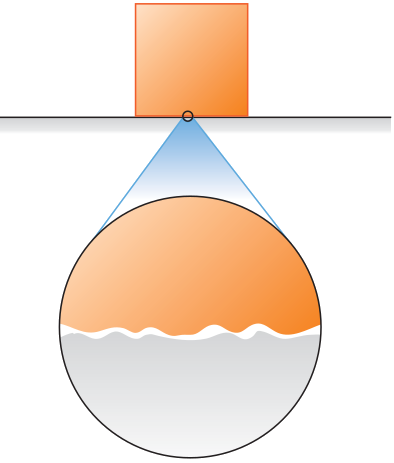
\includegraphics[scale=.3]{friction_block}};
	\node at (1,2) {\ak \text{វត្ថុ}};
	\node at (2.5,1) {\ak \text{ផ្ទៃប៉ះ}};
	\end{tikzpicture}
	\caption{កម្លាំងកកិត}
\end{figure}
\begin{exercise}
	\begin{enumerate}
		\item នៅលើផ្លូវដេកត្រង់មួយរថយន្តដែលមានម៉ាស $m=1$តោន បានចាប់ហ្រ្វាំងដើម្បីឈប់គោរពតាមស្លាកសញ្ញាចរាចរ។ កម្លាំងកកិត $2$ នៃប្រាំងទាំងអស់សមមូលនឹងកម្លាំងថេរតែមួយដែលមានទិសដេកមានទិសដៅផ្ទុយពីចលនារបស់រថយន្ត និងមានតម្លៃ $f=2000\si{\newton}$។ គណនាសំទុះនៃចលនារបស់រថយន្ត។
		\begin{figure}[H]
			\centering
			\begin{tikzpicture}
				\coordinate (O) at (0,0);
				\node at (0,0) {
\includegraphics[scale=.2]{car_driving}};
				\fill[left color = white, right color=white, fill opacity=1, bottom color=gray, top color=gray!40!white] (-2,-.7) rectangle (2,-.5);
			\end{tikzpicture}
		\end{figure}
		\item រថយន្តមួយផ្លាស់ទីដោយល្បឿន $10\si{\metre/\second}$ លើផ្លូវដេកត្រង់រាបស្មើ។ ចាប់ពីពេលពន្លត់ម៉ាស៊ីនរហូតដល់ពេលឈប់ស្ងៀមរថយន្តរត់បានចម្ងាយ $150\si{\metre}$។ តើរថយន្តរត់លើចម្ងាយផ្លូវនេះក្នុងរយៈពេលប៉ុន្មាន? មេគុណកកិតប៉ុន្មាន?(គេមិនគិតកម្លាំងទប់នៃខ្យល់)។ គេឲ្យ $g=9.80\si{\metre/\second^{2}}$។
	\end{enumerate}
\end{exercise}
\section{អនុវត្តន៍ច្បាប់ញូតុន}
\quad នៅចំណុចនេះយើងនឹងសិក្សាអំពីការប្រើ ឬការអនុវត្តច្បាប់ទាំងបីរបស់ ញូតុន ដើម្បីធ្វើការដោះស្រាយលំហាត់ ក៏ដូចជាស្វែងយល់បន្ថែមអំពីបាតុភូតជាក់ស្តែងរបស់លំហាត់។
\subsection{របៀបប្រើច្បាប់ញូតុនដើម្បីដោះស្រាយលំហាត់}
\begin{key}
	ដើម្បីដោះស្រាយលំហាត់ទាក់ទងនិងច្បាប់ញូតុន យើងត្រូវ៖
	\begin{enumerate}
		\item វិភាគប្រធានលំហាត់ និងបាតុភូតរួចគូសរូប
		\item គូសដ្យាក្រាមកម្លាំងក្រៅទាំងអស់ដែលមានអំពើលើអង្គធាតុនីមួយៗ
		\item ទម្លាក់ចំណោលកែងកម្លាំងនីមួយៗលើអ័ក្ស $\left(\overrightarrow{ox}\right)$ និង $\left(\overrightarrow{oy}\right)$
		\item អនុវត្តច្បាប់ ញូតុន ទៅតាមសម្មតិកម្មដែលគេប្រាប់៖
		\begin{itemize}
			\item បើអង្គធាតុមានលំនឹង ឬមានចលនាត្រង់ស្មើៈ យើងត្រូវប្រើច្បាប់ទី១ ញូតុន ពោលគឺ ឲ្យផលបូកនៃវ៉ិចទ័រកម្លាំងទាំងអស់ដែលមានអំពើលើអង្គធាតុស្មើសូន្យ គេសរសេរ $\Sigma\vec{F}=\vec{0}$	
			\item បើអង្គធាតុផ្លាស់ទីដោយសំទុះថេរ ឬមានចលនាត្រង់ប្រែប្រួលស្មើ យើងត្រូវប្រើច្បាប់ទី២ ញូតុន ពោលគឺ ឲ្យផលបូកនៃវ៉ិចទ័រកម្លាំងទាំងអស់ដែលមានអំពើលើអង្គធាតុស្មើនឹង ម៉ាសគុណនឹងសំទុះរបស់វា គេសរសេរ $\Sigma \vec{F}=m\vec{a}$
		\end{itemize}
		\item សរសេរកន្សោមវ៉ិចទ័រខាងលើ ជាម៉ូឌុល
		\item បង្កើតជាសមីការ រួចដោះស្រាយសមីការនោះ ដើម្បីរកអញ្ញាតដែលគេចង់សួររក។
	\end{enumerate}
\end{key}
\subsection{អង្គធាតុរអិលលើប្លង់ទេរ}
\begin{example}
	\begin{enumerate}
		\item ធុងមួយមានម៉ាស $m$ ដាក់លើផ្ទៃរលោង(កកិតអាចចោលបាន)នៃប្លង់ទេ មួយដែលបង្កើតបានមុំ $\theta$ ជាមួយប្លង់ដេកដូចរូបខាងក្រោម។ ចូរសិក្សាចលនារបស់ធុងក្រោយពីវាត្រូវបានគេលែង។
		\item រូបខាងក្រោម មេគុណកកិតស៊ីនេទិចរវាងដុំម៉ាស $A$ នឹងតុស្មើ​ $0.2$។ ដុំម៉ាស $m_{A}=25\si{\kilogram}$ និង $m_{B}=15\si{\kilogram}$។ ម៉ាសខ្សែ ម៉ាសរ៉ក និងកកិតរវាងខ្សែនឹងរ៉កអាចចោលបាន។ សំទុះទំនាញដី $g=9.80\si{\metre/\second^{2}}$
		\begin{enumerate}[k,2]
			\item គូសដ្យាក្រាមកម្លាំងនៃដុំម៉ាសនីមួយៗ។
			\item រកសំទុះនៃដុំម៉ាសនីមួយៗ។
			\item រកតំណឹងខ្សែ។
			\item តើដុំម៉ាសនីមួយៗផ្លាស់ទីបានប្រវែងប៉ុន្មានក្នុងរយៈពេល $3\si{\second}$ ដំបូងក្រោយពេលលែងដុំម៉ាស$B$
		\end{enumerate}
	\end{enumerate}
	\begin{figure}[H]
		\centering
		\begin{subfigure}[b]{0.45\textwidth}
			\begin{tikzpicture}
				\begin{scope}
					\coordinate (A) at (0,2);
					\coordinate (B) at (4,0);
					\coordinate (C) at (0,0);
					\draw (A)--(B)--(C)--cycle;
					\pic [draw, -, "$\theta$", angle eccentricity=1.5, angle radius=1cm] {angle = A--B--C};
					\draw[gray!40!black, line width=2.5pt] (-.2,0)--(4.2,0);
					\fill[left color = white, right color=white, fill opacity=1, bottom color=gray!40!white, top color=gray] (-.2,0) rectangle (4.2,-.2);
					\draw[gray!40!black, fill=cadetgrey,rotate around={-26.5:(1,1.75)}] (0,2.18) rectangle (1,1.55);
					\draw[dashed, gray!40!black,pattern=north west lines,rotate around={-26.5:(1,1.75)}] (3.3,1.55) rectangle (4.3,2.2);
					\draw[|-|] (1.2,2)--(3.1,1);
					\draw[>=Stealth, ->, line width=2pt] (1.3,2.4) to (2,2) node[above] (2,2) {$\vec{a}$};
					\node at (2.5,1.8) {$d$};
				\end{scope}
			\end{tikzpicture}
			\caption{ធុងរអិលលើប្លង់ទេរ}
		\end{subfigure}
		\begin{subfigure}[b]{0.45\textwidth}
			\begin{tikzpicture}[decoration=rope]
				\coordinate (O) at (0,0);
				\node at (O) {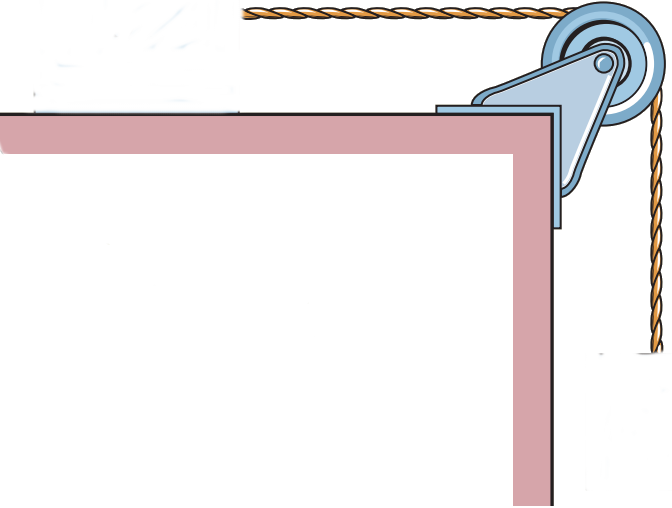
\includegraphics[scale=.18]{pulley_system}};
				\draw[fill=white] (0,1.5) circle (.15cm);
				\filldraw[gray!40!black,fill=cadetgrey] (-1.5,.9) rectangle (0,2.2);
				\node at (-.7,1.5) {$A$};
				\draw[fill=white] (2.05,0) circle (.15cm);
				\filldraw[gray!40!black,fill=cadetgrey] (1.6,-1) rectangle (2.5,0);
				\node at (2.05,-.5) {$B$};
				\draw[>=Stealth, ->, line width=2pt] (2.75, -.5) to (2.75, -1.5) node[right] (3, -1.5) {$\vec{a}$};
				\draw[>=Stealth, ->, line width=2pt] (.5, 1.75) to (1.5, 1.75) node[above] (2, 1.75) {$\vec{a}$};
			\end{tikzpicture}
			\caption{ប្រព័ន្ធរ៉ក}
		\end{subfigure}
	\end{figure}
\end{example}
\newpage
\subsection{ម៉ាស៊ីនអាត់វូត}
\begin{example}
	កាលណាវត្ថុពីរមានម៉ាសមិនស្មើគ្នាចងភ្ជាប់តាមរយៈខ្សែដែលឆ្លងកាត់រ៉ក។ កកិតរវាងរ៉ក និងខ្សែអាចចោលបាន។ ម៉ាសខ្សែ និងម៉ាសរ៉កអាចចោលបាន។ ប្រព័ន្ធដែលបានរៀបរាប់នេះហៅថា ម៉ាស៊ីនអាត់វូត។\\
 	កំណត់សំទុះវត្ថុទាំងពីរ និងតំណឹងខ្សែ។ ចូរអនុវត្តជាលេខបើ $m_{1}=1.0\si{\kilogram},~m_{2}=2.0\si{\kilogram}$ និង $g=9.80\si{\metre/\second^{2}}$។
	\begin{figure}[H]
		\centering
		\begin{tikzpicture}
		\coordinate (O) at (0,0);
		\node at (0,0) {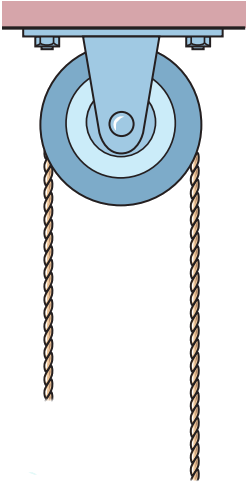
\includegraphics[scale=.25]{pulley}};
		\draw[fill=white] (.65,-2) circle (.15cm);
		\draw[fill=white] (-.65,-.5) circle (.15cm);
		\filldraw[gray!40!black,fill=cadetgrey] (-1.1,-1.5) rectangle (-.2,-.5);
		\filldraw[gray!40!black,fill=cadetgrey] (0,-2) rectangle (1.3,-3.3);
		\node at (-.65,-1) {$m_{1}$};
		\node at (.65,-2.7) {$m_{2}$};
		\draw[>=Stealth, ->, line width=2pt] (-1.7,-1) to (-1.7, .5) node[left] (-1.7, .5) {$\vec{a}$};;
		\draw[>=Stealth, ->, line width=2pt] (1.7, -2.7) to (1.7, -4) node[right] (1.7, -4) {$\vec{a}$};
		\end{tikzpicture}
		\caption{ម៉ាស៊ីនអាត់វូត}
	\end{figure}
\end{example}
\begin{exercise}
	\begin{enumerate}
		\item កម្លាំងពីរមានអំពើលើវត្ថុមួយមានម៉ាស $m=4.0\si{\kilogram}$។ បើ $F_{1}=20.0N$ និង $F_{2}=15.0N$។ ចូរគណនា៖
		\begin{enumerate}[k,2]
			\item កម្លាំងផ្គូបដែលមានអំពើលើវត្ថុនោះ។
			\item គណនាសំទុះនៃវត្ថុនោះ។
		\end{enumerate}
		\item ឈើមួយដុំរាងប្រលេពីប៉ែតកែងបានរអិលដោយគ្មានកកិតចុះតាមបណ្តោយប្លង់ទេ(ដូចរូប)។ មុំរវាងប្លង់ទេរ និងប្លង់ដេកគឺ $\theta=30^\circ$។ ដុំឈើនោះចាប់ផ្តើមផ្លាស់ទីពី $A$ ចុះក្រោមតាមបណ្តោយប្លង់ទេរបានប្រវែង $d=2.0\si{\metre}$។
		\begin{enumerate}
			\item គូសដ្យាក្រាមតាងឲ្យកម្លាំងដែលមានអំពើលើដុំថ្មនោះ។
			\item គណនាសំទុះនៃឈើនោះ។
			\item គណនាល្បឿននៅខណៈដែលដុំឈើនោះមកដល់ចំណុច $B$។ គេយក $g=9.80\si{\metre/\second^2}$។
		\end{enumerate}
	\item អេឡិចត្រុងមួយមានម៉ាស $9.11\times10^{-31}\si{\kilogram}$ ធ្វើចលនាត្រង់ដោយល្បឿនដើម $2.0\times10^{5}\si{\metre/\second}$ និងផ្លាស់ទីបាន $5.0\si{\centi\metre}$។ គេដឹងថាសំទុះនៃអេឡិចត្រុងថេរនិងល្បឿនស្រេចគឺ $6.0\times10^{5}\si{\metre/\second}$។
	\begin{enumerate}
		\item កំណត់កម្លាំងដែលមានអំពើលើអេឡិចត្រុង។
		\item ប្រៀបធៀបកម្លាំងនេះនឹងទម្ងន់របស់អេឡិចត្រុង។ គេឲ្យ $g=9.80\si{\metre/\second^{2}}$។
	\end{enumerate}
	\end{enumerate}
	\begin{figure}[H]
		\centering
		\begin{subfigure}[b]{0.3\textwidth}
			\centering
			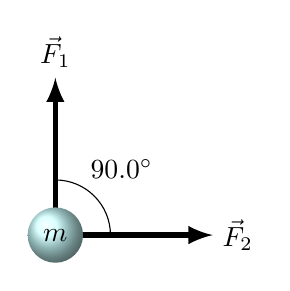
\begin{tikzpicture}
			\begin{scope}
			\coordinate (O) at (0,0);
			\coordinate[label=above:{$\vec{F}_{1}$}] (F2) at (0,2);
			\coordinate[label=right:{$\vec{F}_{2}$}] (F1) at (2,0);
			\draw [->, line width =2pt] (O) -- (F1);
			\draw [->, line width =2pt] (O) -- (F2); 
			\shade [ball color=cyan!20!white] (O) circle [radius=10pt];
			\node at (O) {$m$};
			\pic [draw, "$90.0^\circ$", angle eccentricity=1.7, angle radius=.7cm] {angle= F1--O--F2};
			\end{scope}
			\end{tikzpicture}
			\caption{រូបលំហាត់ទី១}
		\end{subfigure}
		\begin{subfigure}[b]{0.3\textwidth}
			\centering
			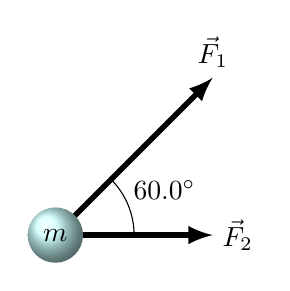
\begin{tikzpicture}
				\begin{scope}
					\coordinate (O) at (0,0);
					\coordinate[label=right:$\vec{F}_{2}$] (F1) at (2,0);
					\coordinate[label=above:$\vec{F}_{1}$] (F2) at (2,2);
					\draw [->, line width =2pt] (O) -- (F1);
					\draw [->, line width =2pt] (O) -- (F2); 
					\shade [ball color=cyan!20!white] (O) circle [radius=10pt];
					\node at (O) {$m$};
					\pic [draw, "$60.0^\circ$", angle eccentricity=1.5, angle radius=1cm] {angle= F1--O--F2};
				\end{scope}
			\end{tikzpicture}
			\caption{រូបលំហាត់ទី១}
		\end{subfigure}
		\begin{subfigure}[b]{0.3\textwidth}
			\centering
			\begin{tikzpicture}
			\begin{scope}
			\coordinate (A) at (0,2);
			\coordinate[label=above right:$B$] (B) at (4,0);
			\coordinate (C) at (0,0);
			\draw (A)--(B)--(C)--cycle;
			\pic [draw, -, "$\theta$", angle eccentricity=1.5, angle radius=1cm] {angle = A--B--C};
			\draw[gray!40!black, line width=2.5pt] (-.2,0)--(4.2,0);
			\fill[left color = white, right color=white, fill opacity=1, bottom color=gray!40!white, top color=gray] (-.2,0) rectangle (4.2,-.2);
			\draw[gray!40!black, fill=cadetgrey,rotate around={-26.5:(1,1.75)}] (0,2.18) rectangle (1,1.55);
			\draw[|-|] (1.2,2)--(4,.6);
			\node at (1.3,2.4) {$A$};
			\node at (2.8,1.5) {$d$};
			\end{scope}
			\end{tikzpicture}
			\caption{រូបលំហាត់ទី២}
		\end{subfigure}
	\end{figure}
\end{exercise}
\end{document}